
%%%%%%%%%%%%%%%%%%%%%%%%%%%%%%%%%%%%%%%%
%\documentclass[review]{cje}
\documentclass[proof]{cje}
%\documentclass{cje}
%%%%%%%%%%%%%%%%%%%%%%%%%%%%%%%%%%%%%%%%

\usepackage{cjenatbib}
\usepackage{url}

\ifx\pdftexversion\undefined
    \usepackage[dvips]{graphicx}
\else
    \usepackage[pdftex]{graphicx}
    \usepackage{epstopdf}
    \epstopdfsetup{suffix=}
\fi

\usepackage{amssymb,amsmath,amsthm}
%\usepackage{pifont}
%\usepackage{mathtools}
%\usepackage{etoolbox}
%\usepackage{subfig}
%\usepackage{txfonts}
%\usepackage{hyperref}
%
%\usepackage{tabularx}
%\usepackage[figuresright]{rotating}
%\usepackage{xcolor}
%\usepackage{floatpag}
%\rotfloatpagestyle{empty}
%\usepackage{lmodern}
%\usepackage{upquote}
%
%\theoremstyle{plain}% default
%\newtheorem{theorem}{Theorem}
%\newtheorem{lemma}{Lemma}
%\newtheorem{proposition}{Proposition}
%\newtheorem*{corollary}{Corollary}
%\theoremstyle{definition}
%\newtheorem{definition}{Definition}
%\newtheorem{example}{Example}
%\theoremstyle{remark}
%\newtheorem*{remark}{Remark}
%\newtheorem*{case}{Case}

% Abbreviations used in this paper.
%\input{Preamble/Notation}
%\input{Preamble/AddNot}

%%%%%%%%%%%%%%%%%%%%%%%%%%%%%%%%%%%%%%%%
\begin{document}
\label{firstpage}
%%%%%%%%%%%%%%%%%%%%%%%%%%%%%%%%%%%%%%%%

\title[Penalties for Speeding and their Effect on Moving Violations]{Penalties for Speeding and their Effect on Moving Violations: Evidence from Quebec Drivers}

\authors{V.~Chandler, L.~Morin, J.~Penney} 

% authors and affiliations

\authorone{Vincent Chandler}{Universit\'{e} du Qu\'{e}bec en Outaouais}

\authortwo{Lealand Morin}{University of Central Florida} 

\authorthree{Jeffrey Penney}{University of Alberta} 

\JEL{K42, K49}

%\acknowledgements{Corresponding author: {\tt KHuynh@Bank-Banque-Canada.ca}.
%                  The views expressed in this paper are those of the authors; 
%		  no responsibility for these views should be attributed to 
%		  the Bank of Canada; all errors are the responsibility of 
%		  the authors.
%
%                  \input{Text/Thanks}
%
%                  }

%%%%%%%%%%%%%%%%%%%%%%%%%%%%%%%%%%%%%%%%

\abstract{

         

In 2008, the province of Quebec drastically increased penalties for speeding 
well above the speed limit by doubling fines and instituting on-the-spot license suspension. 
Using administrative driving and licensing records in Quebec from 2006 to 2010, 
we examine whether the new law discouraged unlawful driving behaviour 
by investigating the frequency with which motorists received traffic citations. 
We find that males became less likely to get traffic tickets after the law came into effect, 
with the largest effects on those aged 16 to 24. 
However, females did not largely change their behaviour in response to this new law. 

\medskip
\noindent
Keywords: driving behaviour, law enforcement, risk aversion, speeding.


         }

%\resume{
%
%        \input{Text/Resume}
%
%       }

%%%%%%%%%%%%%%%%%%%%%%%%%%%%%%%%%%%%%%%%

\maketitle

%%%%%%%%%%%%%%%%%%%%%%%%%%%%%%%%%%%%%%%%

\section{Introduction}
\label{sec:Introduction}

In 2018, 1,743 individuals died in Canada following a car accident 
% (Transport Canada, 2020). 
\citep{transcan2018}. 
Such accidents are the leading cause of death for individuals aged between 15 and 44
% (Statistics Canada, 2020).  
\citep{statscan2020}. 
Many OECD countries have recently introduced harsher punishments to deter the types of behaviour that increase the likelihood of such tragedies. For example, penalties for speeding well above the speed limit now typically include some combination of substantially increased fines, immediate vehicle seizure, and license suspension. These laws are typically referred to as excessive speeding laws or stunt-driving laws.

Quebec followed this trend and introduced excessive speeding penalties in 2008. Its provisions are triggered when driving well above the speed limit. For example, driving at a speed of 100km/h in a 60km/h zone would be considered excessive speeding. These harsher punishments received widespread media coverage both before and after its implementation, and there was a sustained campaign by the provincial government to help ensure drivers were aware of the law. The Quebec government has since declared the legislation to be successful, with the number of excessive speeding tickets decreasing over time. Furthermore, the number of accidents with bodily harm decreased from 36,816 in 2006 to 32,371 in 2010, and the number of accidents with fatalities decreased from 666 to 441 over the same period 
% (SAAQ, 2011). 
% \citep{saaq2011}. 
(\citet{saaq2011}). 
Even though these findings are encouraging, they don’t provide conclusive evidence that the harsher penalties truly caused changes in behaviour. The legislation has been unsuccessfully challenged in court.
Since 
% Becker (1968), 
\citet{becker1968b}, 
economists have theorized that harsher punishments alter the incentives of individuals and thus ultimately their behaviour. 
% Helland and Tabarrok (2007) 
\citet{hellandtabarrok2007} 
provide evidence for this mechanism studying the impact of California’s three-strike legislation on the recidivism rates of felons. However, the effectiveness of deterrence is unclear in the context of driving. Indeed, 
% Bourgeon and Picard (2007) 
\citet{bourgeonpicard2007} 
find that some drivers may be impossible to deter either because they do not care about the penalties or because they are not aware they are speeding.

A broad literature has investigated the role of deterrence on driving and alcohol consumption 
% (e.g. Hansen, 2015), 
(e.g. \citet{hansen2015}), 
but less attention has been devoted to speeding. Some empirical research has determined the impact of very influential policies like the introduction of a demerit point system. For example, 
% Benedettini and Nicita (2009) 
\citet{bennedittiniNicita2009} 
show a reduction in road fatalities through deterrence and incapacitation following the introduction of such a system. More generally, 
% Castillo-Manzano and Castro-Nuño (2012) 
\citet{castillocastro2012} 
provide a meta-study demonstrating the broad positive impact of such a policy in a variety of countries. In Quebec, 
% Dionne et al. (2011) 
\citet{dionneetal2011} 
focus on the threat of the loss of license on the behaviour of a driver close to the demerit point threshold of suspension. They find a reduction in the probability of violation for drivers with a large number of demerit points and conclude the system is successful in deterring the worst offenders.

In this paper, we investigate the effect of Quebec’s excessive speeding legislation on the frequency and types of violations incurred by Quebec drivers using an event-study design. Such violations are a proxy for driving behaviour, so this study will glean insight into the effect of increasing penalties on dangerous driving. It is important to note that we are looking at all violations which result in demerit points, and not just those that are affected by the change in the law. 

We begin with a simple theoretical model to examine the predictions of economic theory on the effect of the law on drivers. The model predicts the possibility of heterogeneous effects by age and gender. We then use driving records obtained from administrative data sets of the Government of Quebec comprising the universe of violations from 2006 to 2010 and records on drivers’ licenses over the same period. The use of large administrative datasets is necessary because only a small fraction of all drivers are impacted by the policy change; yet, these drivers are particularly important because they are generally responsible for accidents causing bodily harm and property damage. We examine the heterogeneous effects of the excessive speeding law on both the extensive (getting a ticket) and the intensive margin (getting a more severe ticket) across gender and age. 

We find that the daily probability of receiving a ticket (extensive margin) decreases after the implementation of the law. When we examine the results by age group, we find that the effects vary substantially, with young drivers between the ages of 16 and 24 being the most affected by the law, while there is little effect for drivers over the age of 45. Repeating the analysis by gender, we see that both males and females change their behaviour, but the magnitude of the effect on males is about eight times that of females. Examining the breakdown by age categories, we see that the effect gradually declines for males until age 55, while there appears to be no age effect for females. 
We then investigate the effect on the intensive margin. For males, the probability of getting tickets worth only one demerit point actually increases following the new policy, while tickets for all other point values decrease. This result suggests that male drivers are still exceeding the speed limit but are driving more slowly than before the introduction of the legislation. A similar pattern exists for female drivers for one and two point violations. We conclude that Quebec’s 2008 excessive speeding law has had substantial spillover effects on both the extensive and intensive margins of driving behaviour. In other words, not only has it reduced the number of drivers driving well above the speed limit, it has also led to a decrease in the propensity to commit other moving violations.

This paper contributes to the literature in several ways. It is the first examination using administrative data into the effect of an excessive speeding law on driving behaviour as proxied by violations by gender and age group. Such analysis is important, because most countries currently use demerit point systems. The question now is not whether these systems work but whether and how they can be adjusted to increase road safety. Moreover, this paper is to our knowledge the first one to empirically investigate the impact of such laws on both the intensive and extensive margins of speeding. Finally, by studying the impact of deterrence by gender and age, this paper fills a gap acknowledged by 
% Freeman (1999) 
\citet{freeman1999}
on the role of gender in studies surrounding criminality.

The rest of this article is organized as follows. Section 2 covers the details of Quebec’s excessive speeding law and the relevant institutional background. A simple theoretical model investigating the effects of the law is constructed in Section 3. The data and summary statistics are presented in Section 4. In Section 5, we conduct the empirical analysis. A series of robustness and placebo checks is conducted in Section 6. We conclude with a policy discussion in Section 7.


\section{Institutional background}
\label{sec:Background}

Vehicular conveyance in the province of Quebec is primarily overseen by a public organization known as the Soci\'{e}t\'{e} de l'assurance automobile du Qu\'{e}bec, commonly abbreviated as SAAQ. This organization was legislated into existence in 1978 and has several mandates. First, it has a public monopoly on the portion of insurance that covers bodily injury. Second, it is responsible for enforcing two key pieces of legislation relating to driving: the Highway Safety Code and the Automobile Insurance Act.\footnote{%
A current list of offences that result in demerit points under the Highway Safety Code can be found at the following web address: \texttt{https://saaq.gouv.qc.ca/en/drivers-licences/demerit-points/offences-and-demerit-points/} (Accessed May 29th, 2020).}
Finally, it manages the driving records of Quebec drivers, including the demerit point system, and the organization promotes road safety through awareness campaigns.

The demerit point system generally operates along the following lines. If a driver is caught committing a violation, the police officer gives the person a ticket according to the violation in question. All violations include a fine and a number of demerit points. Drivers can either admit guilt by paying the ticket or challenge the sanction in court. The violation is recorded in the driver’s file when the guilty plea is received or when the judge convicts the driver. The points are added to the driver’s file when the violation is recorded and remain there for a period of 24 months. If drivers accumulate more than 20 points, they lose their license for at least 3 months after which time they can reapply for one.\footnote{%
This period of time increases every time drivers lose their licence.}
They will only receive a new license if they successfully complete the theoretical and practical driving examinations.

Quebec’s excessive speeding law came into force on April 1st, 2008 and changed the demerit point system managed by the SAAQ. This change was advertised by the SAAQ both before and after the law came into effect. Excessive speeding is defined by the law as exceeding the speed limit by 40 km/h in a zone of 60 km/h or less, by 50 km/h in a zone between 60 to 90 km/h, and by 60 km/h in a zone where the speed limit is equal to or greater than 100 km/h. The law worked in tandem with the then currently legislated speeding violations, increasing fines and demerit point penalties and imposing license suspensions and vehicle seizures. While offences involving demerit points are on a person’s driving record for two years, excessive speeding convictions remain on a person’s driving record for 10 years. The following table details the penalties for violating the excessive speeding law. Note that the license suspension and vehicle seizure occur immediately after being pulled over regardless of the driver’s innocence or guilt, while the fines and demerit points are only entered into the record once the individual admits guilt or is later found guilty in a court of law. \\

\textbf{Table 1 about here} \\



\section{Theoretical Model}
\label{sec:Model}

In this section, we present a simple theoretical model of driving behaviour. We use this to appeal to economic theory to determine whether to expect differences in age and gender as a result of a policy that increases the risk of driving, and if so, whether there would be a pattern in these differences. \\

{\Large There is more...} \\



\section{Data}
\label{sec:Data}


We use records of traffic violations and drivers licenses obtained from SAAQ administrative data to generate a dataset containing the universe of driver-days from April 1st 2006 to March 31st 2010 for the province of Quebec.\footnote{%
The dataset on driver’s licenses allows us to include observations that do not receive any tickets during the sample period.}  
Our dataset contains information on the age, gender, and details concerning traffic violations of the offender. In all, we have approximately 9.7 billion driver-day observations over the sample period. This very large sample will afford us the opportunity to examine detailed subgroups and give us the statistical power to detect effects that are small in absolute magnitude.

We begin with a graphical analysis of some select demerit point values. Here, we examine monthly ticket frequencies for given point values before and after the policy change. Unfortunately, the dataset makes it impossible to distinguish between single and multiple violations for a single police stop. For example, it is impossible to distinguish a driver with two 3-point violations from a driver with a single 6-point violation – all we observe is that both drivers gained 6 demerit points on a given day. Fortunately, multiple violation stops are likely very rare in our sample.\footnote{%
For example, before the excessive speeding law, there were no violations worth 6 points, but the sample shows 517 stops resulting in 6 demerit points compared to 43,006 stops resulting in 5 demerit points. As another example, a single 7-point violation was present before the policy change, but none after; the number of 7-point tickets before the policy change was 8,366, and it decreased to only 24 after the policy change. There are no violations in the Highway Safety Code worth 8 or 11 demerit points at any time in our sample period, and our data shows no stops with demerit point totals of these values.}

Since the demerit point values of some violations have doubled after the excessive speeding law came into effect under certain conditions (see Section 2 for details), we will compare stops associated with a certain number of points before the policy change with those associated with the same number of points and double the number of points after the policy change. For example, a driver speeding 46km/h to 49km/h over the speed limit before the policy change would receive a 5-point ticket, but the same violation would be worth 10 points after the policy change if it qualifies for excessive speeding. Because excessive speeding doubles the point values of some speeding violations, we will need to compare the frequency of 5-point stops before the policy change to 5- or 10-point stops afterwards (as not all 5-point speeding violations may qualify as excessive speeding). Due to the aforementioned possibility of stops with multiple violations, the number of tickets with 5- or 10-point values will contain combinations of violations which will be counted in the post period that were not counted in the pre period, and so the effect of the law will be underestimated in this case, but the overall effect should be minimal.

If drivers do not adjust their behaviour, there should be about as many drivers with 5 points before the policy as there were drivers with 5 or 10 points after the policy. If drivers slow down, the number of 5-point or 10-point violations will decrease. \\

\textbf{Figure 1 about here} \\

Taking into consideration the seasonality of speeding, we see an important reduction in the number of 5- or 10-point tickets in the summer of 2008 than in the preceding summer. Overall, there is a general downward trend in the number of tickets after the policy change compared to before the policy change, and the 5- and 10-point tickets after the change are approximately evenly split. 

With 7- or 14-point stops, we see a different picture: nearly all 7-point violations are worth 14 points after the policy change, while only a few 7-point violations remain. Since there is no violation worth 7 points after the policy change, all of the 7-point stops after the policy change are due to being pulled over for multiple violations totalling 7 points. Once again, we see a downward trend in the number of total violations. \\

\textbf{Figure 2 about here} \\

Table 2 reports summary statistics. Overall, since females represent half of drivers yet only 20\% of traffic violations, they represent a far smaller share of those who receive tickets compared to males. In the 1- and 2-point categories, the number of tickets increases for both males and females on a per driver-day basis, and generally decreases in the higher-point categories, even though more violations lead to an increase of points.

To put these numbers in a broader context, the vast majority of the sample are non-events. Before the excessive speeding law came into effect, the average driver has a probability of 0.04\% to receive a ticket on any particular day. This probability decreases by approximately 3.6\% after the policy change. If we look at the demerit points per driver per day, they decreased after the policy change for males by 6\% and by 1\% for females. This result is particularly interesting, because excessive speeding penalties doubled the value of many speeding violations previously worth 5, 7, and 9 points.\footnote{%  
Some 3-point speeding tickets are subject to the excessive speeding law, but the circumstances are quite particular: the suspect needs to be exceeding the speed limit in a zone with a posted limit of 60km/h or less by 40 to 45 km/h.}
In the absence of a change in behaviour, the number of demerit points per driver per day would have mechanically increased. \\

\textbf{Table 2 about here} \\



\section{Empirical Analysis}
\label{sec:Empirical}


\subsection{Regression results for any moving violation}

We analyze the effect of the excessive speeding law on traffic tickets by means of an event study using a linear probability model. The main regression specification is
\begin{equation}
y_{it} = \beta_0 + \beta_1 d_t
      + \beta_2 d_t agecat_{it} + \beta_3 agecat_{it} + \beta_4 ptsgrp_{it}
      + \epsilon_{it}
\end{equation}

where $d_t$ is a dummy variable equal to 1 after the policy change and 0 before, $agecat$ is a set of age category dummies, $ptsgrp$ is a set of demerit point balance categories, and $\epsilon_it$ is the usual error term.\footnote{% 
Note that the bolded items represent vectors rather than scalars.
}  
The dependent variable y is equal to 1 if the individual received a ticket on that day and 0 otherwise. The age category controls are 16 to 19, 20 to 24, 25 to 34, 35 to 44, 45 to 54, 55 to 64, and 65 and over. The demerit point balance is the sum of demerit points on a driver’s record over the last two years. This variable is divided in to categories of 1 to 3, 4 to 6, 7 to 9, and 10 and over.

Our coefficients of interest are the scalar $\beta_1$ and the vector $\beta_2$. We include the vector $\beta_2$ in some specifications and run some regressions separating by gender because the theoretical model of Section 3 predicted the possibility of heterogeneous effects due to differential attitudes towards risk: females and those of higher ages are likely to be more risk averse. \\

\textbf{Table 3 about here} \\

The regression results are displayed above in Table 3. Due to the very large sample sizes being employed, we elect to only consider statistical significance at the 0.1\% and the 0.001\% level. In the full sample, we see that the imposition of the policy increases the daily probability of receiving a ticket by 0.00382 percentage points, and this is very precisely estimated (t-statistic = -92.992). Once we add the age and policy interactions, the coefficient on the policy dummy is no longer significant, and we see very heterogeneous effects by age group. Most of the effect is concentrated in the 16 to 19 and 20 to 24 age groups, and then the magnitude declines steadily afterwards. The effect loses statistical significance at the 0.1\% level once we reach the 45 to 54 age group.

The theoretical model of Section 3 suggests that the effects differ by gender. We rerun the model using only males and see that the effect increases the daily probability of receiving a ticket by 0.00592 percentage points, an effect 55\% higher than in the pooled sample. Once we add the policy and age group interactions, the coefficient on the policy dummy again becomes insignificant, and the effect appears to be driven by age groups. Examining the coefficients, we see a very distinct pattern: the effect is more or less constant between the ages of 16 and 24, and the effect begins to decline throughout the entire lifecycle, although the effect is no longer significant at the 0.1\% level at the age 55 to 64 age group.\footnote{% 
Be mindful of the change in the exponents in scientific notation as the effect weakens with age, e.g. such as the step from the 20 to 24 age group to the 25 to 34 age group.
}

Conducting the regression for the females in the sample shows that the effect is much smaller for this group: the effect size of the coefficient on the policy dummy is 12.8\% of the size of its counterpart in the regression for males. Once the age interactions are added, none of the coefficients are significant at the elevated 1\% level. These findings suggest that the pooled results are driven almost entirely by males under the age of 55.

It is important to note that the estimate of the effect of the law in the main regression is an average treatment effect; this treatment effect includes drivers who rarely sufficiently exceed the speed limit or otherwise break the law to be penalized with traffic tickets. Assuming these more careful drivers are not affected by the law at all and that they make up a large segment of the population, the effect of the law on the relevant subpopulation that is affected by the law may be well underestimated.


\subsection{Regression results by point total}

In this section, we examine the effects of Quebec’s excessive speeding law by point total. We repeat the policy dummy specification in section 5.1 but restrict the sample to tickets worth 1, 2, 3, 4, 5, 7, and 9 or more points. This strategy will allow us to investigate the changes in the intensive margin of demerit points given to drivers after the policy change. Individuals may substitute driving well above the speed limit with driving at lower speeds but still above the speed limit. As before, the demerit points lost after the policy change take into account the doubling of the penalty due to the excessive speeding law. For example, the 5-point category therefore includes tickets worth 5 points before the policy change and 5 or 10 points after the policy change. These effects might be slightly underestimated (that is, they may have a slight downward bias) since some ticket combinations yielding 10 points after the policy change would be captured by these regressions. However, as previously argued, these sorts of incidents are likely very rare. \\

\textbf{Table 4 about here} \\

We see the results of these regressions by ticket point in Table 4. For males, we see a very minor increase in the number of tickets worth 1 point after the policy change. This increase in 1-point tickets is dwarfed by the decrease in the tickets in all of the other point categories and is alone cancelled out by the decrease in two point tickets. For females, a similar pattern is found in that 1- and 2-point tickets increase slightly, but this increase is more than cancelled out by the decrease in 3-point tickets. There is a decrease in 4-point tickets, but it is not precisely estimated. All ticket values of 5 or more points decrease after the policy change. Note that the coefficient sizes for some of the higher ticket point categories on Table 4 are quite small: this is because high ticket values are rare, and so any decrease in them will have a smaller coefficient, since it represents a change from one small number to another small number.

These patterns suggest that many drivers have decreased their average speed after the policy change. It appears likely that many people who used to speed well above the limit have decreased their speed such that they are still exceeding the limit, but not as much as before. Since the extensive margin of tickets has decreased, it looks like many who used to speed at moderate speeds over the limit are now no longer speeding.


\subsection{Regression results for drivers with high point balances}

It may be of interest to know how drivers who typically drive less carefully (and thus accumulate more demerit points) may have seen their point balances shift on average after the implementation of the policy. We examine the subsample of drivers who at one point in the pre-period had a point balance of between 6 and 10 demerit points. Therefore, two categories of drivers are excluded: those whose point balance never reaches 6 (most of the sample), and those who received serious tickets and therefore whose point balance is never in this range. For example, a person who received a singular ticket for excessive speeding worth 12 demerit points will not be a part of this sample because their point balance will remain at 12 as long as the ticket is on their record, and the balance will drop down to 0 when the ticket’s demerit points expire: at no point was this driver’s demerit point balance between 6 and 10. The results of this exercise by gender are on Table 5 below. \\

\textbf{Table 5 about here} \\

For males, the effect on high point drivers has an interesting pattern by age. The effect is very strong for people age 16 to 19, decreases in the next age group, but then is more or less steady after that. For women, the policy has much less of an effect than for males, and the effect also smoothly decreases with age. Overall, the frequency of tickets decreases by a relatively large margin for this group of drivers after the policy.






\section{Concerns of Validity}
\label{sec:Validity}


\subsection{Alternative explanations for the downturn in tickets}

To rule out any possibility that these results are driven by secular trend, we repeat the regression specified in Section 5.1 by splitting the pre-period in half. Because of the very heterogeneous effects by gender, we perform two sets of placebo checks, one for males and one for females. The results of this analysis are displayed in Table 5. \\

\textbf{Table 6 about here} \\

The regression results show no evidence of pre-trends. In the regressions without the policy and age interactions, the coefficients are not precisely estimated. Moreover, the magnitude of the coefficients in both placebo regressions are almost identical and their magnitude corresponds to approximately one-eighth of those in the real regression for males. If there were a secular trend in the pre-period driving the results of the main regressions, the male coefficient would have a larger magnitude than the female coefficient, but this is not the case. In the set of regressions containing the age category dummies interacted with the policy variable, none of the interactions are statistically significant, and there is no pattern among the coefficients either. This result contrasts with the coefficients on the age interactions for males in the main regression in which we observe a clear pattern: the effect is similar from ages 16 to 25, and then slowly declines with age. Overall, there is no evidence that the effects found in the real regression are an artifact of something other than the excessive speeding laws.

During about the last third of the sample period after the policy change, the province of Quebec introduced a photo radar pilot, which started to distribute tickets for speeding on August 19th, 2009. We do not believe this had a substantial effect on driver behaviour for several reasons. First, the number of photo radar machines was very small: there were 15 in the entire province of Quebec, which had a population of approximately 8 million people at the time.\footnote{% 
Of these 15, 6 were for speeding, 6 were for red light violations, and 3 were mobile 
%(La Presse, 2020).
\citet{bisson2020}.
}  
Second, during the pilot, the photo radar machines were placed in plain sight, and warning signs were placed ahead of them to clearly alert drivers of their location.

An alternative explanation is the idea that police leniency may have changed as a result of the law. We do not believe this is the case. One can assume that the introduction of additional penalties for excessive speeding may motivate police officers to write fewer tickets for these crimes and note them as lesser speeding violations instead, under the assumption that they have a distaste for appearing in court. In Quebec, however, police officers are not required to appear in traffic court.\footnote{% 
See the following website (in French) for details: \texttt{https://educaloi.qc.ca/capsules/la-contestation-dune-contravention/} (Accessed July 18th, 2020).}  
In terms of police behaviour specifically in response to those who speed at a level to obtain excessive speeding penalties under the new regime, it would be reasonable to assume that a police officer aiming to be lenient would reduce the speed on a ticket to a level where the excessive speeding provisions would not take effect. For example, excessive speeding in zones with a limit of 60km/h could be marked down to a 3 point ticket, while excessive speeding in zones with higher limits could be reduced to a 5 point ticket. 

However, according to Table 4, the incidence of tickets for men decreases for every category above 1-point, while for women it decreases for every category above 2 points, and so the categories to which the tickets would be marked down still saw decreases.\footnote{% 
Note that there are no speeding violations worth 4 points under the Quebec highway safety code, and that 4-point tickets are much less common than 3-point or 5-point tickets, see Table 2.
}  
If driving behaviour had not changed and police had become more lenient by marking down speeds below the excessive speeding thresholds, we would see an increase in tickets for the 3 and 5 point categories, which we do not observe in the data. Finally, the overall number of tickets per driver day still decreased (the extensive margin), and leniency against the provisions of the excessive speeding law would only affect the intensive margin of demerit points. We conclude it is very unlikely that a change in police leniency could be driving the results.


\subsection{Statistical properties}

Concerns may be raised about the mathematical properties of estimates derived from the use of linear probability models. For example, 
% Horrace and Oaxaca (2006) 
\citet{horraceoaxaca2006}
claim that predicted probabilities outside of the $[0,1]$ interval are indicative of bias and inconsistency of the linear probability model regression estimates. For all regressions conducted in our paper, no predicted probabilities fall outside of this interval, thus ruling out this possibility. Furthermore, the absence of negative predictions is not a product of chance; the explanatory variables in our regressions are all categorical variables. The predictions are essentially proportions, rather than linear predictions from continuous variables, and this mitigates the usual criticism of the linear probability model. 

Another issue is the relative rarity of the events (the driver-days where the dependent variable is equal 1 rather than 0). 
% King and Zeng (2001) 
\citet{kingzheng2001}
show that rare events cause estimated probabilities to be biased downwards for logit estimation (in the case where ones are rare relative to zeros). The level of the rare events bias is a function of the frequency of events relative to the total sample size: for example, a sample size of 1,000 with 2 events (0.2\% of the sample) may suffer from rare events bias, but a sample size of 100,000 with 200 events (also 0.2\%) may not. To examine whether rare events bias potentially exists in our analysis, we conduct a simulation as follows. We set up a simulation using an effect size that is similar to the regression involving females but uses a much smaller sample size: if rare events bias is absent, it should be absent in the real regression which has a sample 100 times larger. The simulation has 1,000 repetitions. For each, we generate a dataset with 43,390,582 observations where 0.00369\% of observations in the pre-period have an event, and 0.004449\% in the post-period. The effect size of interest is the difference between these two numbers which is 0.000759\%. The results are as follows. We find no evidence of rare events bias: the mean effect size of the simulations is also 0.000759\% and the estimates are tightly distributed, with the 25th percentile being equal to 0.000620\%, and the 75th percentile to 0.000889\%. Moreover, the statistical power is healthy, with 30.1\% of the samples producing statistically significant results for the effect size at the 0.001\% level. This is despite the simulation using a sample size only one one-hundredth that of the sample used in the analysis. We conclude that there is no evidence that rare events bias is influencing the results.



\section{Policy Discussion}
\label{sec:Discussion}


This paper studies the impact of an increase in penalties for speeding. We find a decrease in the number of severe violations, especially for young males. These results offer some important policy implications.

First, we document a significant spillover effect from the introduction of the law. Even though excessive speeding events targeted by the law are relatively rare, the law appears to have influenced many drivers. Indeed, if the only reactions were from people usually speeding well above the speed limit, we would likely not find statistically detectable effects in the overall sample, given the low share of tickets for excessive speeding (see Table 2). Overall, the legislation decreased the number of violations and caused people who habitually drive above the limit to speed less. This spillover effect is somewhat puzzling. Perhaps the excessive speeding law made people more aware of speeding penalties in general. Since drivers do not always pay close attention to their speed, the threat of more severe penalties may have increased their awareness for their speed in more mundane circumstances.

Second, this analysis shows variations in the capacity to deter different groups of individuals. Young males seem to react particularly strongly to such penalties. Since this group is usually responsible for dangerous driving, this type of policy seems to be particularly effective to improve roadway safety.


%\pagebreak
%Gratuitous list of citations goes here: 
%
% \citet{tardiff2010}
% \citet{shi2009}
% \citet{levittmiles2006}
% \citet{levitt1997}
% \citet{klicktabarrock2005}
% \citet{hussetal2006}
% \citet{hellandtabarrok2007}
% \citet{hansen2015}
%\citet{haque1990}
% \citet{evansowens2007}
% \citet{dmw2011}
% \citet{ditellaschar2004}
% \citet{dionneetal2011}
% \citet{deangelohansen2014}
% \citet{bourgeonpicard2007}
% \citet{bennedittiniNicita2009}
% \citet{bjm2014}
%% \citet{becker1968}
% \citet{becker1968a}
% \citet{becker1968b}
% \citet{pulido2010}

% \input{../Text/Acknowledgements}

%%%%%%%%%%%%%%%%%%%%%%%%%%%%%%%%%%%%%%%%

\vfill
\eject

%%%%%%%%%%%%%%%%%%%%%%%%%%%%%%%%%%%%%%%%

\clearpage

% 
\pagebreak

% \section*{Appendix A}
%\section*{Appendix}
%\vspace{3.0in}

% \section*{Tables and Figures from Previous Draft}
%\section*{Appendix: Tables and Figures}
%\label{sec:Appendix}

%\vfill
%\eject


\begin{table}% [ht]
\centering
\begin{tabular}{p{1.5cm} p{1.5cm} p{2cm} p{2.5cm} p{2.5cm}}
  \hline
     				& First  	& Second	& Third 	& Subsequent  \\ 
				& offence	& offence	& offence 	& offences \\
  \hline
Licence suspension
	&  7 days
		& 30 days
			& 60 days if all three offences were committed in a zone of 60km/h or less, 
				otherwise 30 days
				& 60 days if this offence and at least two others were committed 
					in a zone of 60km/h or less, otherwise 30 days \\
   \hline
Vehicle seizure 
	& none
		& 30 days if both offences committed in a zone of 60km/h or less
			& 30 days if this offence and at least one other were committed 
				in a zone of 60km/h or less
				& 30 days if this offence and at least one other were committed 
					in a zone of 60km/h or less \\
   \hline
Fines			& doubled			& doubled			& doubled			& doubled \\
   \hline
Demerit Points	& doubled			& doubled			& doubled			& tripled \\
   \hline
\end{tabular}
\caption{Penalties for Excessive Speeding} 
\label{tab:penalties}
\end{table}

\begin{figure}
\centering
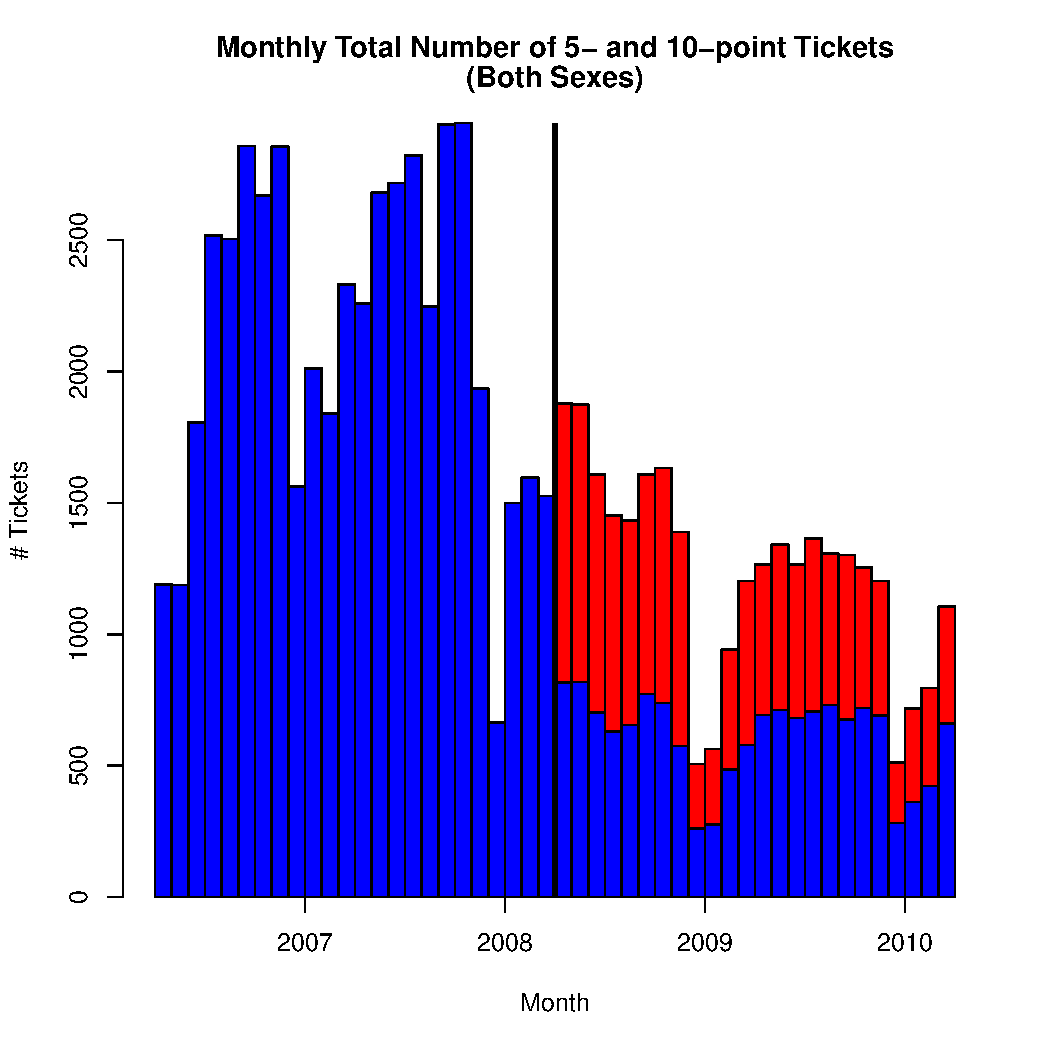
\includegraphics[width=0.8\textwidth]{../Figures/num_pts_5_10_all_orig.pdf}
\caption{Monthly frequency of 5- and 10-point violations }
Notes: Authors calculations. Monthly frequency of 5-point violations before the policy change and 5- or 10-point violations after the policy change. Blue areas correspond to 5 point-stops, while red areas are 10-point stops.
\label{fig:num_pts_5_10_all}
\end{figure}


\begin{figure}
\centering
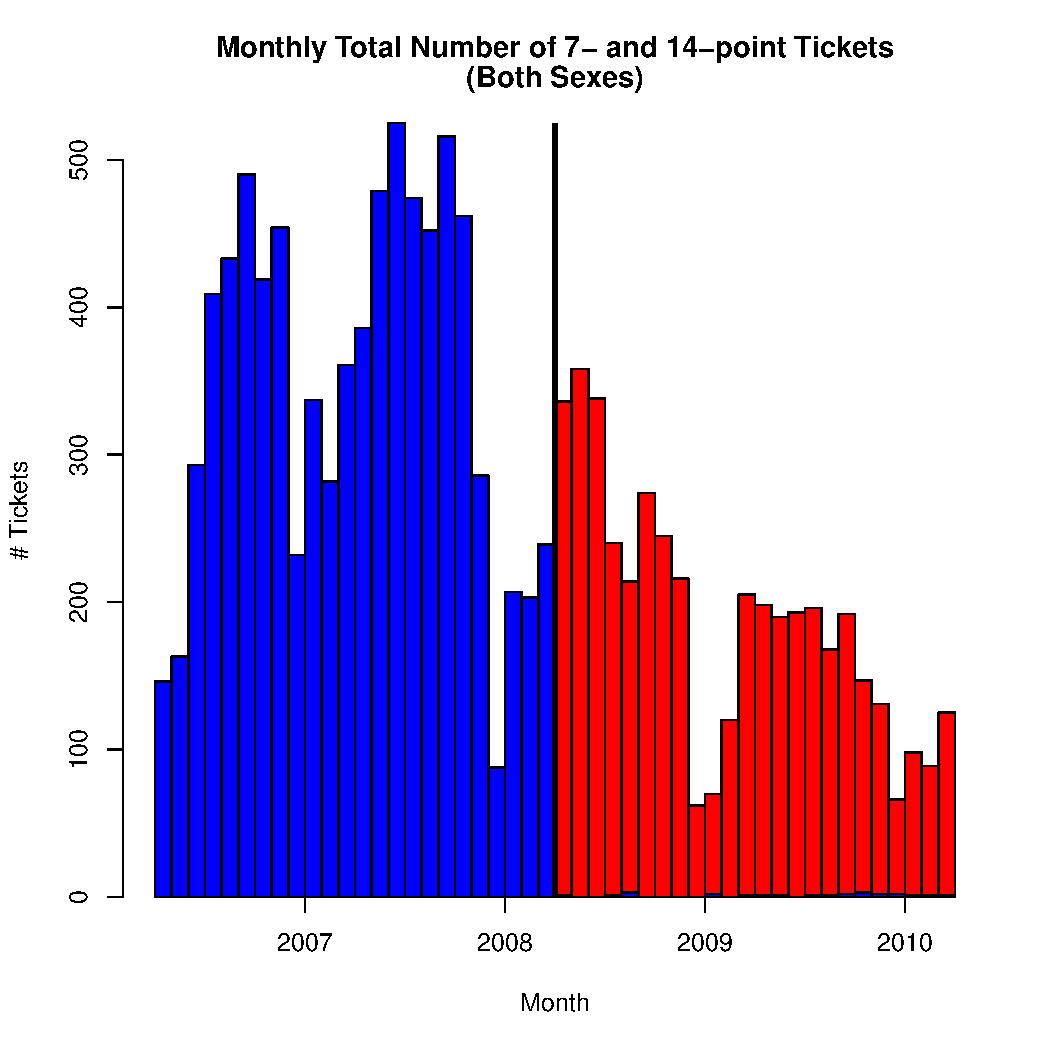
\includegraphics[width=0.8\textwidth]{../Figures/num_pts_7_14_all_orig.pdf}
\caption{Monthly frequency of 5- and 10-point violations }
Notes: Authors calculations. Monthly frequency of 7-point violations before the policy change and 7- or 14-point violations after the policy change. Blue areas correspond to 7-point stops, while red areas are 14-point stops.
\label{fig:num_pts_7_14_all}
\end{figure}



% 
\begin{table}% [ht]
\centering
\begin{tabular}{r r r r r r r}
  \hline
		& \multicolumn{2}{c}{Both} 	&  \multicolumn{2}{c}{Males} &  \multicolumn{2}{c}{Females} \\
  \hline
points 	& pre 			& post			& pre 			& post			& pre 			& post		\\ 
  \hline

1		& 146,680		& 184,677		& 101,298		& 122,899		& 45,382		& 61,778    \\
2		& 782,836		& 855,302		& 533,167		& 572,194		& 249,669		& 283,108    \\
3		& 949,044		& 867,361		& 701,053		& 627,807		& 247,991		& 239,554    \\
4		& 17,783		& 17,748		& 15,567		& 15,278		& 2,216		& 2,470    \\
5		& 51,178		& 14,640		& 43,006		& 12,368		& 8,172		& 2,272    \\
6		& 517			& 15,296		& 496			& 12,000		& 21			& 3,296    \\
7		& 8,336		& 24			& 7,688		& 18			& 648			& 6    \\
9		& 9,969		& 8,222		& 7,382		& 5,791		& 2,587		& 2,431    \\
10		& 0				& 14,884		& 0				& 12,747		& 0				& 2,137    \\
12		& 128			& 0				& 127			& 0				& 1				& 0    \\
14		& 0				& 4,447		& 0				& 4,145		& 0				& 302    \\
15		& 18			& 0				& 17			& 0				& 1				& 0    \\
18		& 3				& 583			& 3				& 560			& 0				& 23    \\
24		& 0				& 102			& 0				& 98			& 0				& 4    \\
30		& 0				& 17			& 0				& 17			& 0				& 0    \\
36		& 0				& 4				& 0				& 4				& 0				& 0    \\

   \hline
Total 	& 1,966,492 	& 1,983,307 	& 1,409,804 	& 1,385,926 	& 556,688 		& 597,381 \\ 
   \hline
\end{tabular}
\caption{Frequency of tickets by point value} 
Notes: Author’s calculations. The pre and post columns refer to before and after the policy change.
\label{tab:penalties}
\end{table}


\begin{table}% [ht]
\centering
\begin{tabular}{r r r r r r r}
  \hline
		& \multicolumn{2}{c}{Male Drivers} 	&  \multicolumn{2}{c}{Female Drivers} &  \multicolumn{2}{c}{Gender Ratio} \\
 & & & & & \multicolumn{2}{c}{(Percent Males)} \\

 \cmidrule(lr){2-3}\cmidrule(lr){4-5}\cmidrule(lr){6-7} 
%  \hline
Points 	& Pre 		& Post		& Pre 		& Post		& Pre 		& Post		\\ 
  \hline
1 		& 101,298 	& 122,899	&  45,382 	&   61,778 	& 69\% 	& 67\% \\ 
2 		& 533,167 	& 572,194	& 249,669 	& 283,108 	& 68\% 	& 67\% \\ 
3 		& 701,053 	& 627,807	& 247,991	& 239,554	& 74\% 	& 72\% \\ 
4 		&  15,567 	&  15,278 	&    2,216 	&    2,470 	& 88\% 	& 86\% \\ 
5 		&  43,006 	&  12,368 	&    8,172 	&    2,272 	& 84\% 	& 84\% \\ 
6 		&     496 	&  12,000 	&        21 	&    3,296 	& 96\% 	& 78\% \\ 
7 		&   7,688 	&        18 	&      648 	&          6 	& 92\% 	& 75\% \\ 
9 		&   7,382 	&    5,791 	&    2,587 	&    2,431 	& 74\% 	& 70\% \\ 
10 		&         0 	&  12,747 	&         0 	&    2,137 	& -			& 86\% \\ 
12 		&     127	&         0 	&         1 	&         0 	& 99\% 	& - \\ 
14 		&       0 	&   4,145 	&         0 	&      302 	& -			& 93\% \\ 
15 		&      17 	&         0 	&         1 	&         0 	& 94\% 	& - \\ 
18 		&       3 	&      560 	&         0 	&        23 	& 100\% 	& 96\% \\ 
24 		&       0 	&       98 	&         0 	&         4 	& -			& 96\% \\ 
30 		&       0 	&       17 	&         0 	&         0 	& -			& 100\% \\ 
36 		&       0 	&        4 	&         0 	&         0 	& -			& 100\% \\ 

   \hline

Total 	  & 1,409,804 & 1,385,926 & 556,688 & 597,381 & 72 & 70 \\ 

   \hline
\end{tabular}
\caption{Frequency of tickets by point value} 
The headings ``Pre'' and ``Post'' columns refer to offences that occurred before and after the policy change. 
The gender ratio is measured as the percentage of the number of offences committed by males 
divided by the total number of offences committed by all drivers. 
\label{tab:point_freq}
\end{table}
% 
\begin{table}% [ht]
\centering
\begin{tabular}{r r r r r r r r r}
  \hline
		& \multicolumn{2}{c}{All Drivers} 	& \multicolumn{2}{c}{Male Drivers} 	&  \multicolumn{2}{c}{Female Drivers} &  \multicolumn{2}{c}{Gender Ratio} \\
 & & & & & & & \multicolumn{2}{c}{(Percent Males)} \\

 \cmidrule(lr){2-3}\cmidrule(lr){4-5}\cmidrule(lr){6-7} 
%  \hline
Points 	& Pre 			& Post			& Pre 		& Post		& Pre 		& Post		& Pre 	& Post		\\ 
  \hline
1		& 146,680		& 184,677		& 101,298 	& 122,899	&  45,382 	&   61,778 	& 69 	& 67 \\ 
2		& 782,836		& 855,302		& 533,167 	& 572,194	& 249,669 	& 283,108 	& 68 	& 67 \\ 
3		& 949,044		& 867,361		& 701,053 	& 627,807	& 247,991	& 239,554	& 74 	& 72 \\ 
4		& 17,783		& 17,748		&  15,567 	&  15,278 	&    2,216 	&    2,470 	& 88 	& 86 \\ 
5		& 51,178		& 14,640		&  43,006 	&  12,368 	&    8,172 	&    2,272 	& 84 	& 84 \\ 
6		& 517			& 15,296		&     496 	&  12,000 	&        21 	&    3,296 	& 96 	& 78 \\ 
7		& 8,336		& 24			&   7,688 	&        18 	&      648 	&          6 	& 92 	& 75 \\ 
9		& 9,969		& 8,222		&   7,382 	&    5,791 	&    2,587 	&    2,431 	& 74 	& 70 \\ 
10		& 0				& 14,884		&         0 	&  12,747 	&         0 	&    2,137 	&  		& 86 \\ 
12		& 128			& 0				&     127	&         0 	&         1 	&         0 	& 99 	&  \\ 
14		& 0				& 4,447		&       0 	&   4,145 	&         0 	&      302 	&  		& 93 \\ 
15		& 18			& 0				&      17 	&         0 	&         1 	&         0 	& 94 	&  \\ 
18		& 3				& 583			&       3 	&      560 	&         0 	&        23 	& 100 	& 96 \\ 
24		& 0				& 102			&       0 	&       98 	&         0 	&         4 	&  		& 96 \\ 
30		& 0				& 17			&       0 	&       17 	&         0 	&         0 	&  		& 100 \\ 
36		& 0				& 4				&       0 	&        4 	&         0 	&         0 	&  		& 100 \\ 

   \hline

Total 	& 1,966,492 	& 1,983,307 	& 1,409,804 & 1,385,926 & 556,688 & 597,381 & 72 & 70 \\ 

   \hline
\end{tabular}
\caption{Frequency of tickets by point value} 
Notes: Author’s calculations. The headings ``Pre'' and ``Post'' columns refer to offences that ocurred before and after the policy change.
\label{tab:penalties}
\end{table}




%% Linear Probability Models: Original Specification 

\begin{table}% [ht] 
\centering 
\begin{tabular}{l r r l r r l} 

\hline 
 
 
 

\hline  

\end{tabular} 
\caption{Regressions} 
\label{tab:orig_regs} 
\end{table} 
 

%
%% Linear Probability Models: Original LPM Specification by Point Value 

\begin{table}% [ht] 
\centering 
\begin{tabular}{l r r l r r l} 

\hline 
 
 & \multicolumn{3}{c}{Males} & \multicolumn{3}{c}{Females} \\ 

\hline 
 
 & Estimate & Std. Error & Sig. & Estimate & Std. Error & Sig. \\ 

\hline 
 
All point values                &  -5.92E-05        &  6.28E-07       &   **       &  -7.59E-06        &  4.95E-07       &   **       \\ 
1 points                        &  3.98E-06        &  1.77E-07       &   **       &  5.22E-06        &  1.50E-07       &   **       \\ 
2 points                        &  -4.11E-06        &  3.94E-07       &   **       &  3.81E-06        &  3.36E-07       &   **       \\ 
3 points                        &  -4.76E-05        &  4.36E-07       &   **       &  -1.41E-05        &  3.23E-07       &   **       \\ 
4 points                        &  -8.09E-07        &  6.62E-08       &   **       &  -1.01E-08        &  3.16E-08       &            \\ 
5 points                        &  -8.20E-06        &  9.95E-08       &   **       &  -2.11E-06        &  5.27E-08       &   **       \\ 
7 points                        &  -1.63E-06        &  4.17E-08       &   **       &  -1.92E-07        &  1.47E-08       &   **       \\ 
9 or more points                &  -6.75E-07        &  4.47E-08       &   **       &  -1.78E-07        &  3.29E-08       &   **       \\ 
Observations            & 5,335,033,221    &          &              &  4,340,212,273 \\ 


\hline 

\end{tabular} 
\caption{Regressions by ticket-point value (Original LPM)} 
All regressions contain age category and demerit point category controls. 
The symbol * denotes statistical significance at the 0.1\% level 
and ** the 0.001\% level. 
``Sig.'' is an abbreviation for statistical significance. 
Estimates and standard errors are in scientific notation. 
Heteroskedasticity-robust errors are employed. 
The baseline age category comprises drivers under the age of 16. 
The 5 point category of tickets includes 10 point tickets after the policy change,  
the 7 point category includes 14 point tickets after the policy change,  
and 9 or more point tickets include all possible doubled values for those tickets  
worth more than 9 points after the policy change. 
\label{tab:orig_regs_by_points} 
\end{table} 
 

%
%% Linear Probability Models: Original High-Point Subsample 

\begin{table}% [ht] 
\centering 
\begin{tabular}{l r r l r r l} 

\hline 
 
 & Estimate & Std. Error & Sig. & Estimate & Std. Error & Sig. \\ 

\hline 
 
\textbf{Full sample} \\ 

Policy             &  -3.82E-05        &  4.11E-07       &   **       &  -1.12E-05        &  5.70E-06       &            \\ 
Age 16-19 * policy           & & &  &  -6.28E-05        &  6.71E-06       &   **       \\ 
Age 20-24 * policy           & & &  &  -6.81E-05        &  6.06E-06       &   **       \\ 
Age 25-34 * policy           & & &  &  -5.17E-05        &  5.81E-06       &   **       \\ 
Age 35-44 * policy           & & &  &  -2.70E-05        &  5.78E-06       &   **       \\ 
Age 45-54 * policy           & & &  &  -1.96E-05        &  5.76E-06       &    *       \\ 
Age 55-64 * policy           & & &  &  -1.23E-05        &  5.76E-06       &            \\ 
Age 65+ * policy           & & &  &  3.59E-06        &  5.75E-06       &            \\ 
Observations & 1,170,426,426 \\ 


\hline 

\textbf{Male} \\ 

Policy             &  -5.92E-05        &  6.28E-07       &   **       &  -1.04E-05        &  7.34E-06       &            \\ 
Age 16-19 * policy           & & &  &  -1.12E-04        &  9.19E-06       &   **       \\ 
Age 20-24 * policy           & & &  &  -1.20E-04        &  8.02E-06       &   **       \\ 
Age 25-34 * policy           & & &  &  -8.63E-05        &  7.54E-06       &   **       \\ 
Age 35-44 * policy           & & &  &  -5.04E-05        &  7.48E-06       &   **       \\ 
Age 45-54 * policy           & & &  &  -3.58E-05        &  7.45E-06       &   **       \\ 
Age 55-64 * policy           & & &  &  -2.53E-05        &  7.46E-06       &    *       \\ 
Age 65+ * policy           & & &  &  -2.91E-06        &  7.43E-06       &            \\ 
Observations & 921,131,812 \\ 


\hline 

\textbf{Female} \\ 

Policy             &  -7.59E-06        &  4.95E-07       &   **       &  -6.70E-06        &  6.35E-06       &            \\ 
Age 16-19 * policy           & & &  &  7.47E-06        &  7.41E-06       &            \\ 
Age 20-24 * policy           & & &  &  -8.99E-07        &  6.76E-06       &            \\ 
Age 25-34 * policy           & & &  &  -9.93E-06        &  6.48E-06       &            \\ 
Age 35-44 * policy           & & &  &  1.57E-07        &  6.46E-06       &            \\ 
Age 45-54 * policy           & & &  &  -2.16E-06        &  6.42E-06       &            \\ 
Age 55-64 * policy           & & &  &  9.92E-07        &  6.42E-06       &            \\ 
Age 65+ * policy           & & &  &  9.38E-06        &  6.42E-06       &            \\ 
Observations & 249,294,614 \\ 


\hline 

\end{tabular} 
\caption{Regressions for high-point drivers} 
All regressions contain age category and demerit point category controls. 
The symbol * denotes statistical significance at the 0.1\% level 
and ** the 0.001\% level. 
``Sig.'' is an abbreviation for statistical significance. 
Estimates and standard errors are in scientific notation. 
Heteroskedasticity-robust errors are employed. 
The baseline age category comprises drivers under the age of 16. 
\label{tab:orig_high_pt_regs} 
\end{table} 
 

%
%% Linear Probability Models: Original LPM Specification for High-Point Drivers by Point Value 

\begin{table}% [ht] 
\centering 
\begin{tabular}{l r r l r r l} 

\hline 
 
 & \multicolumn{3}{c}{Males} & \multicolumn{3}{c}{Females} \\ 

\hline 
 
 & Estimate & Std. Error & Sig. & Estimate & Std. Error & Sig. \\ 

\hline 
 
All point values                &  -3.79E-04        &  2.11E-06       &   **       &  -2.59E-04        &  3.15E-06       &   **       \\ 
1 points                        &  -5.33E-06        &  5.72E-07       &   **       &  -8.08E-07        &  8.30E-07       &            \\ 
2 points                        &  -7.66E-05        &  1.26E-06       &   **       &  -5.85E-05        &  1.97E-06       &   **       \\ 
3 points                        &  -2.44E-04        &  1.52E-06       &   **       &  -1.76E-04        &  2.25E-06       &   **       \\ 
4 points                        &  -8.42E-06        &  2.05E-07       &   **       &  -2.42E-06        &  1.81E-07       &   **       \\ 
5 points                        &  -3.32E-05        &  3.93E-07       &   **       &  -1.64E-05        &  4.69E-07       &   **       \\ 
7 points                        &  -7.26E-06        &  1.73E-07       &   **       &  -2.02E-06        &  1.51E-07       &   **       \\ 
9 or more points                &  -3.54E-06        &  1.45E-07       &   **       &  -2.56E-06        &  2.02E-07       &   **       \\ 
Observations            & 921,131,812    &          &              &  249,294,614 \\ 


\hline 

\end{tabular} 
\caption{Regressions for high-point drivers by ticket-point value (Original LPM)} 
All regressions contain age category and demerit point category controls. 
The symbol * denotes statistical significance at the 0.1\% level 
and ** the 0.001\% level. 
``Sig.'' is an abbreviation for statistical significance. 
Estimates and standard errors are in scientific notation. 
Heteroskedasticity-robust errors are employed. 
The baseline age category comprises drivers under the age of 16. 
The 5 point category of tickets includes 10 point tickets after the policy change,  
the 7 point category includes 14 point tickets after the policy change,  
and 9 or more point tickets include all possible doubled values for those tickets  
worth more than 9 points after the policy change. 
\label{tab:orig_regs_by_points} 
\end{table} 
 

%
%% Linear Probability Models: Original Placebo Specification 

\begin{table}% [ht] 
\centering 
\begin{tabular}{l r r l r r l} 

\hline 
 
 & Estimate & Std. Error & Sig. & Estimate & Std. Error & Sig. \\ 

\hline 
 
\textbf{Full sample} \\ 

Policy             &  -3.87E-06        &  5.92E-07       &   **       &  -1.29E-05        &  8.06E-06       &            \\ 
Age 16-19 * policy           & & &  &  -1.91E-05        &  9.61E-06       &            \\ 
Age 20-24 * policy           & & &  &  9.64E-07        &  8.59E-06       &            \\ 
Age 25-34 * policy           & & &  &  6.16E-06        &  8.21E-06       &            \\ 
Age 35-44 * policy           & & &  &  4.05E-06        &  8.17E-06       &            \\ 
Age 45-54 * policy           & & &  &  1.15E-05        &  8.14E-06       &            \\ 
Age 55-64 * policy           & & &  &  1.51E-05        &  8.15E-06       &            \\ 
Age 65+ * policy           & & &  &  1.96E-05        &  8.14E-06       &            \\ 
Observations & 4,728,750,336 \\ 


\hline 

\textbf{Male} \\ 

Policy             &  -2.01E-06        &  9.06E-07       &            &  -1.80E-05        &  1.02E-05       &            \\ 
Age 16-19 * policy           & & &  &  -2.94E-05        &  1.31E-05       &            \\ 
Age 20-24 * policy           & & &  &  -1.01E-06        &  1.12E-05       &            \\ 
Age 25-34 * policy           & & &  &  1.34E-05        &  1.05E-05       &            \\ 
Age 35-44 * policy           & & &  &  1.24E-05        &  1.04E-05       &            \\ 
Age 45-54 * policy           & & &  &  1.98E-05        &  1.04E-05       &            \\ 
Age 55-64 * policy           & & &  &  2.33E-05        &  1.04E-05       &            \\ 
Age 65+ * policy           & & &  &  2.73E-05        &  1.03E-05       &            \\ 
Observations & 2,618,869,394 \\ 


\hline 

\textbf{Female} \\ 

Policy             &  -1.73E-06        &  7.07E-07       &            &  7.30E-06        &  9.25E-06       &            \\ 
Age 16-19 * policy           & & &  &  -1.16E-05        &  1.08E-05       &            \\ 
Age 20-24 * policy           & & &  &  -1.14E-06        &  9.82E-06       &            \\ 
Age 25-34 * policy           & & &  &  -1.06E-05        &  9.44E-06       &            \\ 
Age 35-44 * policy           & & &  &  -1.51E-05        &  9.40E-06       &            \\ 
Age 45-54 * policy           & & &  &  -8.68E-06        &  9.35E-06       &            \\ 
Age 55-64 * policy           & & &  &  -6.71E-06        &  9.36E-06       &            \\ 
Age 65+ * policy           & & &  &  -3.47E-06        &  9.34E-06       &            \\ 
Observations & 2,109,880,942  \\ 


\hline 

\end{tabular} 
\caption{Placebo regressions} 
All regressions contain age category and demerit point category controls. 
The symbol * denotes statistical significance at the 0.1\% level 
and ** the 0.001\% level. 
``Sig.'' is an abbreviation for statistical significance. 
Estimates and standard errors are in scientific notation. 
Heteroskedasticity-robust errors are employed. 
The baseline age category comprises drivers under the age of 16. 
\label{tab:orig_placebo_regs} 
\end{table} 
 

%
%
%
%\clearpage
%\pagebreak
%
%\section*{Appendix B}
%\vspace{3.0in}
%
%\section*{Tables with Seasonality}
%% \label{sec:Appendix}
%
%\vfill
%\eject
%
%% Linear Probability Models: Seasonal LPM Specification 

\begin{table}% [ht] 
\centering 
\begin{tabular}{l r r l r r l} 

\hline 
 
 & Estimate & Std. Error & Sig. & Estimate & Std. Error & Sig. \\ 

\hline 
 
\textbf{Full sample} \\ 

Policy             &  -3.87E-05        &  4.11E-07       &   **       &  -1.18E-05        &  5.70E-06       &            \\ 
Age 16-19 * policy           & & &  &  -6.27E-05        &  6.71E-06       &   **       \\ 
Age 20-24 * policy           & & &  &  -6.77E-05        &  6.06E-06       &   **       \\ 
Age 25-34 * policy           & & &  &  -5.15E-05        &  5.81E-06       &   **       \\ 
Age 35-44 * policy           & & &  &  -2.68E-05        &  5.78E-06       &   **       \\ 
Age 45-54 * policy           & & &  &  -1.95E-05        &  5.76E-06       &    *       \\ 
Age 55-64 * policy           & & &  &  -1.22E-05        &  5.76E-06       &            \\ 
Age 65+ * policy           & & &  &  3.77E-06        &  5.75E-06       &            \\ 
Observations & 9,675,245,494 \\ 


\hline 

\textbf{Male} \\ 

Policy             &  -5.97E-05        &  6.28E-07       &   **       &  -1.09E-05        &  7.34E-06       &            \\ 
Age 16-19 * policy           & & &  &  -1.12E-04        &  9.19E-06       &   **       \\ 
Age 20-24 * policy           & & &  &  -1.19E-04        &  8.02E-06       &   **       \\ 
Age 25-34 * policy           & & &  &  -8.62E-05        &  7.54E-06       &   **       \\ 
Age 35-44 * policy           & & &  &  -5.03E-05        &  7.48E-06       &   **       \\ 
Age 45-54 * policy           & & &  &  -3.57E-05        &  7.45E-06       &   **       \\ 
Age 55-64 * policy           & & &  &  -2.52E-05        &  7.46E-06       &    *       \\ 
Age 65+ * policy           & & &  &  -2.81E-06        &  7.43E-06       &            \\ 
Observations & 5,335,033,221 \\ 


\hline 

\textbf{Female} \\ 

Policy             &  -8.00E-06        &  4.95E-07       &   **       &  -7.47E-06        &  6.35E-06       &            \\ 
Age 16-19 * policy           & & &  &  7.80E-06        &  7.41E-06       &            \\ 
Age 20-24 * policy           & & &  &  -4.42E-07        &  6.77E-06       &            \\ 
Age 25-34 * policy           & & &  &  -9.59E-06        &  6.48E-06       &            \\ 
Age 35-44 * policy           & & &  &  5.31E-07        &  6.46E-06       &            \\ 
Age 45-54 * policy           & & &  &  -1.83E-06        &  6.42E-06       &            \\ 
Age 55-64 * policy           & & &  &  1.34E-06        &  6.42E-06       &            \\ 
Age 65+ * policy           & & &  &  9.73E-06        &  6.42E-06       &            \\ 
Observations & 4,340,212,273 \\ 


\hline 

\end{tabular} 
\caption{Regressions (Seasonal LPM)} 
All regressions contain age category and demerit point category controls. 
The symbol * denotes statistical significance at the 0.1\% level 
and ** the 0.001\% level. 
``Sig.'' is an abbreviation for statistical significance. 
Estimates and standard errors are in scientific notation. 
Heteroskedasticity-robust errors are employed. 
The baseline age category comprises drivers under the age of 16. 
\label{tab:seas_regs} 
\end{table} 
 

%
%% Linear Probability Models: Seasonal LPM Specification by Point Value 

\begin{table}% [ht] 
\centering 
\begin{tabular}{l r r l r r l} 

\hline 
 
 & \multicolumn{3}{c}{Males} & \multicolumn{3}{c}{Females} \\ 

\hline 
 
 & Estimate & Std. Error & Sig. & Estimate & Std. Error & Sig. \\ 

\hline 
 
All point values                &  -5.97E-05        &  6.28E-07       &   **       &  -8.00E-06        &  4.95E-07       &   **       \\ 
1 points                        &  3.93E-06        &  1.77E-07       &   **       &  5.17E-06        &  1.50E-07       &   **       \\ 
2 points                        &  -4.32E-06        &  3.94E-07       &   **       &  3.61E-06        &  3.36E-07       &   **       \\ 
3 points                        &  -4.78E-05        &  4.36E-07       &   **       &  -1.43E-05        &  3.23E-07       &   **       \\ 
4 points                        &  -8.04E-07        &  6.62E-08       &   **       &  -1.03E-08        &  3.16E-08       &            \\ 
5 points                        &  -8.19E-06        &  9.95E-08       &   **       &  -2.10E-06        &  5.27E-08       &   **       \\ 
7 points                        &  -1.62E-06        &  4.17E-08       &   **       &  -1.91E-07        &  1.47E-08       &   **       \\ 
9 or more points                &  -6.75E-07        &  4.47E-08       &   **       &  -1.80E-07        &  3.29E-08       &   **       \\ 
Observations            & 5,335,033,221    &          &              &  4,340,212,273 \\ 


\hline 

\end{tabular} 
\caption{Regressions by ticket-point value (Seasonal LPM)} 
All regressions contain age category and demerit point category controls. 
The symbol * denotes statistical significance at the 0.1\% level 
and ** the 0.001\% level. 
``Sig.'' is an abbreviation for statistical significance. 
Estimates and standard errors are in scientific notation. 
Heteroskedasticity-robust errors are employed. 
The baseline age category comprises drivers under the age of 16. 
The 5 point category of tickets includes 10 point tickets after the policy change,  
the 7 point category includes 14 point tickets after the policy change,  
and 9 or more point tickets include all possible doubled values for those tickets  
worth more than 9 points after the policy change. 
\label{tab:seas_regs_by_points} 
\end{table} 
 

%
%% Linear Probability Models: Seasonal LPM High-Point Subsample 

\begin{table}% [ht] 
\centering 
\begin{tabular}{l r r l r r l} 

\hline 
 
 & Estimate & Std. Error & Sig. & Estimate & Std. Error & Sig. \\ 

\hline 
 
\textbf{Full sample} \\ 

Policy             &  -3.87E-05        &  4.11E-07       &   **       &  -1.18E-05        &  5.70E-06       &            \\ 
Age 16-19 * policy           & & &  &  -6.27E-05        &  6.71E-06       &   **       \\ 
Age 20-24 * policy           & & &  &  -6.77E-05        &  6.06E-06       &   **       \\ 
Age 25-34 * policy           & & &  &  -5.15E-05        &  5.81E-06       &   **       \\ 
Age 35-44 * policy           & & &  &  -2.68E-05        &  5.78E-06       &   **       \\ 
Age 45-54 * policy           & & &  &  -1.95E-05        &  5.76E-06       &    *       \\ 
Age 55-64 * policy           & & &  &  -1.22E-05        &  5.76E-06       &            \\ 
Age 65+ * policy           & & &  &  3.77E-06        &  5.75E-06       &            \\ 
Observations & 1,170,426,426 \\ 


\hline 

\textbf{Male} \\ 

Policy             &  -5.97E-05        &  6.28E-07       &   **       &  -1.09E-05        &  7.34E-06       &            \\ 
Age 16-19 * policy           & & &  &  -1.12E-04        &  9.19E-06       &   **       \\ 
Age 20-24 * policy           & & &  &  -1.19E-04        &  8.02E-06       &   **       \\ 
Age 25-34 * policy           & & &  &  -8.62E-05        &  7.54E-06       &   **       \\ 
Age 35-44 * policy           & & &  &  -5.03E-05        &  7.48E-06       &   **       \\ 
Age 45-54 * policy           & & &  &  -3.57E-05        &  7.45E-06       &   **       \\ 
Age 55-64 * policy           & & &  &  -2.52E-05        &  7.46E-06       &    *       \\ 
Age 65+ * policy           & & &  &  -2.81E-06        &  7.43E-06       &            \\ 
Observations & 921,131,812 \\ 


\hline 

\textbf{Female} \\ 

Policy             &  -8.00E-06        &  4.95E-07       &   **       &  -7.47E-06        &  6.35E-06       &            \\ 
Age 16-19 * policy           & & &  &  7.80E-06        &  7.41E-06       &            \\ 
Age 20-24 * policy           & & &  &  -4.42E-07        &  6.77E-06       &            \\ 
Age 25-34 * policy           & & &  &  -9.59E-06        &  6.48E-06       &            \\ 
Age 35-44 * policy           & & &  &  5.31E-07        &  6.46E-06       &            \\ 
Age 45-54 * policy           & & &  &  -1.83E-06        &  6.42E-06       &            \\ 
Age 55-64 * policy           & & &  &  1.34E-06        &  6.42E-06       &            \\ 
Age 65+ * policy           & & &  &  9.73E-06        &  6.42E-06       &            \\ 
Observations & 249,294,614 \\ 


\hline 

\end{tabular} 
\caption{Regressions for high-point drivers (Seasonal LPM)} 
All regressions contain age category and demerit point category controls. 
The symbol * denotes statistical significance at the 0.1\% level 
and ** the 0.001\% level. 
``Sig.'' is an abbreviation for statistical significance. 
Estimates and standard errors are in scientific notation. 
Heteroskedasticity-robust errors are employed. 
The baseline age category comprises drivers under the age of 16. 
\label{tab:seas_high_pt_regs} 
\end{table} 
 

%
%% Linear Probability Models: Seasonal LPM Specification for High-Point Drivers by Point Value 

\begin{table}% [ht] 
\centering 
\begin{tabular}{l r r l r r l} 

\hline 
 
 & \multicolumn{3}{c}{Males} & \multicolumn{3}{c}{Females} \\ 

\hline 
 
 & Estimate & Std. Error & Sig. & Estimate & Std. Error & Sig. \\ 

\hline 
 
All point values                &  -3.81E-04        &  2.11E-06       &   **       &  -2.60E-04        &  3.15E-06       &   **       \\ 
1 points                        &  -5.45E-06        &  5.72E-07       &   **       &  -9.16E-07        &  8.30E-07       &            \\ 
2 points                        &  -7.71E-05        &  1.26E-06       &   **       &  -5.90E-05        &  1.97E-06       &   **       \\ 
3 points                        &  -2.45E-04        &  1.52E-06       &   **       &  -1.77E-04        &  2.25E-06       &   **       \\ 
4 points                        &  -8.45E-06        &  2.05E-07       &   **       &  -2.42E-06        &  1.81E-07       &   **       \\ 
5 points                        &  -3.32E-05        &  3.93E-07       &   **       &  -1.64E-05        &  4.69E-07       &   **       \\ 
7 points                        &  -7.27E-06        &  1.73E-07       &   **       &  -2.02E-06        &  1.51E-07       &   **       \\ 
9 or more points                &  -3.54E-06        &  1.45E-07       &   **       &  -2.57E-06        &  2.02E-07       &   **       \\ 
Observations            & 921,131,812    &          &              &  249,294,614 \\ 


\hline 

\end{tabular} 
\caption{Regressions for high-point drivers by ticket-point value (Seasonal LPM)} 
All regressions contain age category and demerit point category controls. 
The symbol * denotes statistical significance at the 0.1\% level 
and ** the 0.001\% level. 
``Sig.'' is an abbreviation for statistical significance. 
Estimates and standard errors are in scientific notation. 
Heteroskedasticity-robust errors are employed. 
The baseline age category comprises drivers under the age of 16. 
The 5 point category of tickets includes 10 point tickets after the policy change,  
the 7 point category includes 14 point tickets after the policy change,  
and 9 or more point tickets include all possible doubled values for those tickets  
worth more than 9 points after the policy change. 
\label{tab:seas_regs_by_points} 
\end{table} 
 

%
%% Linear Probability Models: Seasonal LPM Placebo Specification 

\begin{table}% [ht] 
\centering 
\begin{tabular}{l r r l r r l} 

\hline 
 
 & Estimate & Std. Error & Sig. & Estimate & Std. Error & Sig. \\ 

\hline 
 
\textbf{Full sample} \\ 

Policy             &  -3.96E-06        &  5.92E-07       &   **       &  -1.31E-05        &  8.06E-06       &            \\ 
Age 16-19 * policy           & & &  &  -1.90E-05        &  9.61E-06       &            \\ 
Age 20-24 * policy           & & &  &  1.04E-06        &  8.59E-06       &            \\ 
Age 25-34 * policy           & & &  &  6.23E-06        &  8.21E-06       &            \\ 
Age 35-44 * policy           & & &  &  4.12E-06        &  8.17E-06       &            \\ 
Age 45-54 * policy           & & &  &  1.16E-05        &  8.14E-06       &            \\ 
Age 55-64 * policy           & & &  &  1.52E-05        &  8.15E-06       &            \\ 
Age 65+ * policy           & & &  &  1.97E-05        &  8.14E-06       &            \\ 
Observations & 4,728,750,336 \\ 


\hline 

\textbf{Male} \\ 

Policy             &  -2.11E-06        &  9.05E-07       &            &  -1.81E-05        &  1.02E-05       &            \\ 
Age 16-19 * policy           & & &  &  -2.94E-05        &  1.31E-05       &            \\ 
Age 20-24 * policy           & & &  &  -1.00E-06        &  1.12E-05       &            \\ 
Age 25-34 * policy           & & &  &  1.34E-05        &  1.05E-05       &            \\ 
Age 35-44 * policy           & & &  &  1.24E-05        &  1.04E-05       &            \\ 
Age 45-54 * policy           & & &  &  1.98E-05        &  1.04E-05       &            \\ 
Age 55-64 * policy           & & &  &  2.33E-05        &  1.04E-05       &            \\ 
Age 65+ * policy           & & &  &  2.73E-05        &  1.03E-05       &            \\ 
Observations & 2,618,869,394 \\ 


\hline 

\textbf{Female} \\ 

Policy             &  -1.80E-06        &  7.06E-07       &            &  6.98E-06        &  9.25E-06       &            \\ 
Age 16-19 * policy           & & &  &  -1.13E-05        &  1.08E-05       &            \\ 
Age 20-24 * policy           & & &  &  -9.14E-07        &  9.82E-06       &            \\ 
Age 25-34 * policy           & & &  &  -1.04E-05        &  9.44E-06       &            \\ 
Age 35-44 * policy           & & &  &  -1.49E-05        &  9.40E-06       &            \\ 
Age 45-54 * policy           & & &  &  -8.44E-06        &  9.36E-06       &            \\ 
Age 55-64 * policy           & & &  &  -6.45E-06        &  9.36E-06       &            \\ 
Age 65+ * policy           & & &  &  -3.17E-06        &  9.34E-06       &            \\ 
Observations & 2,109,880,942  \\ 


\hline 

\end{tabular} 
\caption{Placebo regressions (Seasonal LPM)} 
All regressions contain age category and demerit point category controls. 
The symbol * denotes statistical significance at the 0.1\% level 
and ** the 0.001\% level. 
``Sig.'' is an abbreviation for statistical significance. 
Estimates and standard errors are in scientific notation. 
Heteroskedasticity-robust errors are employed. 
The baseline age category comprises drivers under the age of 16. 
\label{tab:seas_placebo_regs} 
\end{table} 
 

%
%
%
%
%\clearpage
%\pagebreak
%
%\section*{Appendix C}
%\vspace{3.0in}
%
%\section*{Tables with Seasonality (Logistic)}
%% \label{sec:Appendix}
%
%\vfill
%\eject
%
%% Logistic Regression Models: Seasonal Logit Specification 

\begin{table}% [ht] 
\centering 
\begin{tabular}{l r r l r r l} 

\hline 
 
 & Estimate & Std. Error & Sig. & Estimate & Std. Error & Sig. \\ 

\hline 
 
\textbf{Full sample} \\ 

Policy             &  -0.0926        &  0.0010       &   **       &  -0.0435        &  0.0370       &            \\ 
Age 16-19 * policy           & & &  &  -0.0684        &  0.0373       &            \\ 
Age 20-24 * policy           & & &  &  -0.0822        &  0.0371       &            \\ 
Age 25-34 * policy           & & &  &  -0.0834        &  0.0370       &            \\ 
Age 35-44 * policy           & & &  &  -0.0430        &  0.0371       &            \\ 
Age 45-54 * policy           & & &  &  -0.0337        &  0.0371       &            \\ 
Age 55-64 * policy           & & &  &  -0.0225        &  0.0371       &            \\ 
Age 65+ * policy           & & &  &  0.0385        &  0.0372       &            \\ 
Observations & 9,675,245,494 \\ 


\hline 

\textbf{Male} \\ 

Policy             &  -0.1113        &  0.0012       &   **       &  -0.0195        &  0.0386       &            \\ 
Age 16-19 * policy           & & &  &  -0.1107        &  0.0389       &            \\ 
Age 20-24 * policy           & & &  &  -0.1300        &  0.0387       &    *       \\ 
Age 25-34 * policy           & & &  &  -0.1301        &  0.0387       &    *       \\ 
Age 35-44 * policy           & & &  &  -0.0891        &  0.0387       &            \\ 
Age 45-54 * policy           & & &  &  -0.0713        &  0.0387       &            \\ 
Age 55-64 * policy           & & &  &  -0.0594        &  0.0387       &            \\ 
Age 65+ * policy           & & &  &  0.0011        &  0.0389       &            \\ 
Observations & 5,335,033,221 \\ 


\hline 

\textbf{Female} \\ 

Policy             &  -0.0294        &  0.0019       &   **       &  -0.0760        &  0.1304       &            \\ 
Age 16-19 * policy           & & &  &  0.0625        &  0.1307       &            \\ 
Age 20-24 * policy           & & &  &  0.0415        &  0.1305       &            \\ 
Age 25-34 * policy           & & &  &  0.0200        &  0.1304       &            \\ 
Age 35-44 * policy           & & &  &  0.0508        &  0.1304       &            \\ 
Age 45-54 * policy           & & &  &  0.0450        &  0.1304       &            \\ 
Age 55-64 * policy           & & &  &  0.0587        &  0.1305       &            \\ 
Age 65+ * policy           & & &  &  0.1335        &  0.1306       &            \\ 
Observations & 4,340,212,273 \\ 


\hline 

\end{tabular} 
\caption{Regressions (Seasonal Logit)} 
All regressions contain age category and demerit point category controls. 
The symbol * denotes statistical significance at the 0.1\% level 
and ** the 0.001\% level. 
``Sig.'' is an abbreviation for statistical significance. 
Estimates and standard errors are in general number format. 
Logistic regression model. 
The baseline age category comprises drivers under the age of 16. 
\label{tab:seas_logit_regs} 
\end{table} 
 

%
%% Logistic Regression Models: Seasonal Logit Specification by Point Value 

\begin{table}% [ht] 
\centering 
\begin{tabular}{l r r l r r l} 

\hline 
 
 & \multicolumn{3}{c}{Males} & \multicolumn{3}{c}{Females} \\ 

\hline 
 
 & Estimate & Std. Error & Sig. & Estimate & Std. Error & Sig. \\ 

\hline 
 
All point values                &  -0.1113        &  0.0012       &   **       &  -0.0294        &  0.0019       &   **       \\ 
1 points                        &  0.0953        &  0.0043       &   **       &  0.2124        &  0.0062       &   **       \\ 
2 points                        &  -0.0191        &  0.0019       &   **       &  0.0303        &  0.0028       &   **       \\ 
3 points                        &  -0.1872        &  0.0017       &   **       &  -0.1256        &  0.0029       &   **       \\ 
4 points                        &  -0.1252        &  0.0114       &   **       &  -0.0098        &  0.0293       &            \\ 
5 points                        &  -0.6470        &  0.0080       &   **       &  -0.7494        &  0.0187       &   **       \\ 
7 points                        &  -0.7392        &  0.0193       &   **       &  -0.9113        &  0.0695       &   **       \\ 
9 or more points                &  -0.2501        &  0.0170       &   **       &  -0.1541        &  0.0282       &   **       \\ 
Observations            & 5,335,033,221    &          &              &  4,340,212,273 \\ 


\hline 

\end{tabular} 
\caption{Regressions by ticket-point value (Seasonal Logit)} 
All regressions contain age category and demerit point category controls. 
The symbol * denotes statistical significance at the 0.1\% level 
and ** the 0.001\% level. 
``Sig.'' is an abbreviation for statistical significance. 
Estimates and standard errors are in general number format. 
Logistic regression model. 
The baseline age category comprises drivers under the age of 16. 
The 5 point category of tickets includes 10 point tickets after the policy change,  
the 7 point category includes 14 point tickets after the policy change,  
and 9 or more point tickets include all possible doubled values for those tickets  
worth more than 9 points after the policy change. 
\label{tab:seas_logit_regs_by_points} 
\end{table} 
 

%
%% Logistic Regression Models: Seasonal Logit High-Point Subsample 

\begin{table}% [ht] 
\centering 
\begin{tabular}{l r r l r r l} 

\hline 
 
 & Estimate & Std. Error & Sig. & Estimate & Std. Error & Sig. \\ 

\hline 
 
\textbf{Full sample} \\ 

Policy             &  -0.0926        &  0.0010       &   **       &  -0.0435        &  0.0370       &            \\ 
Age 16-19 * policy           & & &  &  -0.0684        &  0.0373       &            \\ 
Age 20-24 * policy           & & &  &  -0.0822        &  0.0371       &            \\ 
Age 25-34 * policy           & & &  &  -0.0834        &  0.0370       &            \\ 
Age 35-44 * policy           & & &  &  -0.0430        &  0.0371       &            \\ 
Age 45-54 * policy           & & &  &  -0.0337        &  0.0371       &            \\ 
Age 55-64 * policy           & & &  &  -0.0225        &  0.0371       &            \\ 
Age 65+ * policy           & & &  &  0.0385        &  0.0372       &            \\ 
Observations & 1,170,426,426 \\ 


\hline 

\textbf{Male} \\ 

Policy             &  -0.1113        &  0.0012       &   **       &  -0.0195        &  0.0386       &            \\ 
Age 16-19 * policy           & & &  &  -0.1107        &  0.0389       &            \\ 
Age 20-24 * policy           & & &  &  -0.1300        &  0.0387       &    *       \\ 
Age 25-34 * policy           & & &  &  -0.1301        &  0.0387       &    *       \\ 
Age 35-44 * policy           & & &  &  -0.0891        &  0.0387       &            \\ 
Age 45-54 * policy           & & &  &  -0.0713        &  0.0387       &            \\ 
Age 55-64 * policy           & & &  &  -0.0594        &  0.0387       &            \\ 
Age 65+ * policy           & & &  &  0.0011        &  0.0389       &            \\ 
Observations & 921,131,812 \\ 


\hline 

\textbf{Female} \\ 

Policy             &  -0.0294        &  0.0019       &   **       &  -0.0760        &  0.1304       &            \\ 
Age 16-19 * policy           & & &  &  0.0625        &  0.1307       &            \\ 
Age 20-24 * policy           & & &  &  0.0415        &  0.1305       &            \\ 
Age 25-34 * policy           & & &  &  0.0200        &  0.1304       &            \\ 
Age 35-44 * policy           & & &  &  0.0508        &  0.1304       &            \\ 
Age 45-54 * policy           & & &  &  0.0450        &  0.1304       &            \\ 
Age 55-64 * policy           & & &  &  0.0587        &  0.1305       &            \\ 
Age 65+ * policy           & & &  &  0.1335        &  0.1306       &            \\ 
Observations & 249,294,614 \\ 


\hline 

\end{tabular} 
\caption{Regressions for high-point drivers (Seasonal Logit)} 
All regressions contain age category and demerit point category controls. 
The symbol * denotes statistical significance at the 0.1\% level 
and ** the 0.001\% level. 
``Sig.'' is an abbreviation for statistical significance. 
Estimates and standard errors are in general number format. 
Logistic regression model. 
The baseline age category comprises drivers under the age of 16. 
\label{tab:seas_logit_high_pt_regs} 
\end{table} 
 

%
%% Logistic Regression Models: Seasonal Logit Specification for High-Point Drivers by Point Value 

\begin{table}% [ht] 
\centering 
\begin{tabular}{l r r l r r l} 

\hline 
 
 & \multicolumn{3}{c}{Males} & \multicolumn{3}{c}{Females} \\ 

\hline 
 
 & Estimate & Std. Error & Sig. & Estimate & Std. Error & Sig. \\ 

\hline 
 
All point values                &  -0.3732        &  0.0021       &   **       &  -0.4252        &  0.0052       &   **       \\ 
1 points                        &  -0.0735        &  0.0076       &   **       &  -0.0239        &  0.0193       &            \\ 
2 points                        &  -0.2111        &  0.0035       &   **       &  -0.2441        &  0.0082       &   **       \\ 
3 points                        &  -0.4677        &  0.0029       &   **       &  -0.5749        &  0.0075       &   **       \\ 
4 points                        &  -0.8975        &  0.0228       &   **       &  -1.2986        &  0.1060       &   **       \\ 
5 points                        &  -1.0016        &  0.0124       &   **       &  -1.3612        &  0.0425       &   **       \\ 
7 points                        &  -1.1495        &  0.0291       &   **       &  -1.6962        &  0.1444       &   **       \\ 
9 or more points                &  -0.7647        &  0.0319       &   **       &  -1.1624        &  0.0942       &   **       \\ 
Observations            & 921,131,812    &          &              &  249,294,614 \\ 


\hline 

\end{tabular} 
\caption{Regressions for high-point drivers by ticket-point value (Seasonal Logit)} 
All regressions contain age category and demerit point category controls. 
The symbol * denotes statistical significance at the 0.1\% level 
and ** the 0.001\% level. 
``Sig.'' is an abbreviation for statistical significance. 
Estimates and standard errors are in general number format. 
Logistic regression model. 
The baseline age category comprises drivers under the age of 16. 
The 5 point category of tickets includes 10 point tickets after the policy change,  
the 7 point category includes 14 point tickets after the policy change,  
and 9 or more point tickets include all possible doubled values for those tickets  
worth more than 9 points after the policy change. 
\label{tab:seas_logit_regs_by_points} 
\end{table} 
 

%
%% Logistic Regression Models: Seasonal Logit Placebo Specification 

\begin{table}% [ht] 
\centering 
\begin{tabular}{l r r l r r l} 

\hline 
 
 & Estimate & Std. Error & Sig. & Estimate & Std. Error & Sig. \\ 

\hline 
 
\textbf{Full sample} \\ 

Policy             &  -0.0080        &  0.0014       &   **       &  -0.0531        &  0.0519       &            \\ 
Age 16-19 * policy           & & &  &  -0.0102        &  0.0523       &            \\ 
Age 20-24 * policy           & & &  &  0.0199        &  0.0520       &            \\ 
Age 25-34 * policy           & & &  &  0.0354        &  0.0520       &            \\ 
Age 35-44 * policy           & & &  &  0.0345        &  0.0520       &            \\ 
Age 45-54 * policy           & & &  &  0.0581        &  0.0520       &            \\ 
Age 55-64 * policy           & & &  &  0.0777        &  0.0521       &            \\ 
Age 65+ * policy           & & &  &  0.1227        &  0.0522       &            \\ 
Observations & 4,728,750,336 \\ 


\hline 

\textbf{Male} \\ 

Policy             &  -0.0024        &  0.0017       &            &  -0.0572        &  0.0540       &            \\ 
Age 16-19 * policy           & & &  &  -0.0106        &  0.0545       &            \\ 
Age 20-24 * policy           & & &  &  0.0204        &  0.0542       &            \\ 
Age 25-34 * policy           & & &  &  0.0457        &  0.0542       &            \\ 
Age 35-44 * policy           & & &  &  0.0496        &  0.0542       &            \\ 
Age 45-54 * policy           & & &  &  0.0698        &  0.0542       &            \\ 
Age 55-64 * policy           & & &  &  0.0879        &  0.0543       &            \\ 
Age 65+ * policy           & & &  &  0.1316        &  0.0545       &            \\ 
Observations & 2,618,869,394 \\ 


\hline 

\textbf{Female} \\ 

Policy             &  -0.0059        &  0.0027       &            &  0.1696        &  0.1874       &            \\ 
Age 16-19 * policy           & & &  &  -0.1940        &  0.1879       &            \\ 
Age 20-24 * policy           & & &  &  -0.1686        &  0.1875       &            \\ 
Age 25-34 * policy           & & &  &  -0.1848        &  0.1875       &            \\ 
Age 35-44 * policy           & & &  &  -0.1970        &  0.1875       &            \\ 
Age 45-54 * policy           & & &  &  -0.1681        &  0.1875       &            \\ 
Age 55-64 * policy           & & &  &  -0.1496        &  0.1876       &            \\ 
Age 65+ * policy           & & &  &  -0.1028        &  0.1878       &            \\ 
Observations & 2,109,880,942  \\ 


\hline 

\end{tabular} 
\caption{Placebo regressions (Seasonal Logit)} 
All regressions contain age category and demerit point category controls. 
The symbol * denotes statistical significance at the 0.1\% level 
and ** the 0.001\% level. 
``Sig.'' is an abbreviation for statistical significance. 
Estimates and standard errors are in general number format. 
Logistic regression model. 
The baseline age category comprises drivers under the age of 16. 
\label{tab:seas_logit_placebo_regs} 
\end{table} 
 

%
%
%\clearpage
%\pagebreak
%
%\section*{Appendix D}
%\vspace{3.0in}
%
%\section*{Tables with Seasonality (LPM, multiplied by 100,000)}
%% \label{sec:Appendix}
%
%\vfill
%\eject
%
%% Linear Probability Models: Seasonal LPM x 100K Specification 

\begin{table}% [ht] 
\centering 
\begin{tabular}{l r r l r r l} 

\hline 
 
 & Estimate & Std. Error & Sig. & Estimate & Std. Error & Sig. \\ 

\hline 
 
\textbf{Full sample} \\ 

Policy             &  -3.8656        &  0.0411       &   **       &  -1.1761        &  0.5700       &            \\ 
Age 16-19 * policy           & & &  &  -6.2697        &  0.6707       &   **       \\ 
Age 20-24 * policy           & & &  &  -6.7723        &  0.6059       &   **       \\ 
Age 25-34 * policy           & & &  &  -5.1489        &  0.5805       &   **       \\ 
Age 35-44 * policy           & & &  &  -2.6807        &  0.5780       &   **       \\ 
Age 45-54 * policy           & & &  &  -1.9497        &  0.5759       &    *       \\ 
Age 55-64 * policy           & & &  &  -1.2160        &  0.5762       &            \\ 
Age 65+ * policy           & & &  &  0.3767        &  0.5752       &            \\ 
Observations & 9,675,245,494 \\ 


\hline 

\textbf{Male} \\ 

Policy             &  -5.9663        &  0.0628       &   **       &  -1.0915        &  0.7342       &            \\ 
Age 16-19 * policy           & & &  &  -11.1587        &  0.9191       &   **       \\ 
Age 20-24 * policy           & & &  &  -11.9225        &  0.8017       &   **       \\ 
Age 25-34 * policy           & & &  &  -8.6158        &  0.7536       &   **       \\ 
Age 35-44 * policy           & & &  &  -5.0295        &  0.7484       &   **       \\ 
Age 45-54 * policy           & & &  &  -3.5740        &  0.7450       &   **       \\ 
Age 55-64 * policy           & & &  &  -2.5200        &  0.7455       &    *       \\ 
Age 65+ * policy           & & &  &  -0.2808        &  0.7427       &            \\ 
Observations & 5,335,033,221 \\ 


\hline 

\textbf{Female} \\ 

Policy             &  -0.8000        &  0.0495       &   **       &  -0.7470        &  0.6348       &            \\ 
Age 16-19 * policy           & & &  &  0.7804        &  0.7413       &            \\ 
Age 20-24 * policy           & & &  &  -0.0442        &  0.6765       &            \\ 
Age 25-34 * policy           & & &  &  -0.9585        &  0.6483       &            \\ 
Age 35-44 * policy           & & &  &  0.0531        &  0.6458       &            \\ 
Age 45-54 * policy           & & &  &  -0.1831        &  0.6424       &            \\ 
Age 55-64 * policy           & & &  &  0.1339        &  0.6424       &            \\ 
Age 65+ * policy           & & &  &  0.9727        &  0.6416       &            \\ 
Observations & 4,340,212,273 \\ 


\hline 

\end{tabular} 
\caption{Regressions (Seasonal LPM x 100K)} 
All regressions contain age category and demerit point category controls. 
The symbol * denotes statistical significance at the 0.1\% level 
and ** the 0.001\% level. 
``Sig.'' is an abbreviation for statistical significance. 
Estimates and standard errors are multiplied by 100,000. 
Heteroskedasticity-robust errors are employed. 
The baseline age category comprises drivers under the age of 16. 
\label{tab:seas_LPMx100K_regs} 
\end{table} 
 

%
%% Linear Probability Models: Seasonal LPM x 100K Specification by Point Value 

\begin{table}% [ht] 
\centering 
\begin{tabular}{l r r l r r l} 

\hline 
 
 & \multicolumn{3}{c}{Males} & \multicolumn{3}{c}{Females} \\ 

\hline 
 
 & Estimate & Std. Error & Sig. & Estimate & Std. Error & Sig. \\ 

\hline 
 
All point values                &  -5.9663        &  0.0628       &   **       &  -0.8000        &  0.0495       &   **       \\ 
1 points                        &  0.3930        &  0.0177       &   **       &  0.5174        &  0.0150       &   **       \\ 
2 points                        &  -0.4315        &  0.0394       &   **       &  0.3613        &  0.0336       &   **       \\ 
3 points                        &  -4.7786        &  0.0436       &   **       &  -1.4289        &  0.0323       &   **       \\ 
4 points                        &  -0.0804        &  0.0066       &   **       &  -0.0010        &  0.0032       &            \\ 
5 points                        &  -0.8189        &  0.0100       &   **       &  -0.2105        &  0.0053       &   **       \\ 
7 points                        &  -0.1625        &  0.0042       &   **       &  -0.0191        &  0.0015       &   **       \\ 
9 or more points                &  -0.0675        &  0.0045       &   **       &  -0.0180        &  0.0033       &   **       \\ 
Observations            & 5,335,033,221    &          &              &  4,340,212,273 \\ 


\hline 

\end{tabular} 
\caption{Regressions by ticket-point value (Seasonal LPM x 100K)} 
All regressions contain age category and demerit point category controls. 
The symbol * denotes statistical significance at the 0.1\% level 
and ** the 0.001\% level. 
``Sig.'' is an abbreviation for statistical significance. 
Estimates and standard errors are multiplied by 100,000. 
Heteroskedasticity-robust errors are employed. 
The baseline age category comprises drivers under the age of 16. 
The 5 point category of tickets includes 10 point tickets after the policy change,  
the 7 point category includes 14 point tickets after the policy change,  
and 9 or more point tickets include all possible doubled values for those tickets  
worth more than 9 points after the policy change. 
\label{tab:seas_LPMx100K_regs_by_points} 
\end{table} 
 

%
%% Linear Probability Models: Seasonal LPM x 100K High-Point Subsample 

\begin{table}% [ht] 
\centering 
\begin{tabular}{l r r l r r l} 

\hline 
 
 & Estimate & Std. Error & Sig. & Estimate & Std. Error & Sig. \\ 

\hline 
 
\textbf{Full sample} \\ 

Policy             &  -3.8656        &  0.0411       &   **       &  -1.1761        &  0.5700       &            \\ 
Age 16-19 * policy           & & &  &  -6.2697        &  0.6707       &   **       \\ 
Age 20-24 * policy           & & &  &  -6.7723        &  0.6059       &   **       \\ 
Age 25-34 * policy           & & &  &  -5.1489        &  0.5805       &   **       \\ 
Age 35-44 * policy           & & &  &  -2.6807        &  0.5780       &   **       \\ 
Age 45-54 * policy           & & &  &  -1.9497        &  0.5759       &    *       \\ 
Age 55-64 * policy           & & &  &  -1.2160        &  0.5762       &            \\ 
Age 65+ * policy           & & &  &  0.3767        &  0.5752       &            \\ 
Observations & 1,170,426,426 \\ 


\hline 

\textbf{Male} \\ 

Policy             &  -5.9663        &  0.0628       &   **       &  -1.0915        &  0.7342       &            \\ 
Age 16-19 * policy           & & &  &  -11.1587        &  0.9191       &   **       \\ 
Age 20-24 * policy           & & &  &  -11.9225        &  0.8017       &   **       \\ 
Age 25-34 * policy           & & &  &  -8.6158        &  0.7536       &   **       \\ 
Age 35-44 * policy           & & &  &  -5.0295        &  0.7484       &   **       \\ 
Age 45-54 * policy           & & &  &  -3.5740        &  0.7450       &   **       \\ 
Age 55-64 * policy           & & &  &  -2.5200        &  0.7455       &    *       \\ 
Age 65+ * policy           & & &  &  -0.2808        &  0.7427       &            \\ 
Observations & 921,131,812 \\ 


\hline 

\textbf{Female} \\ 

Policy             &  -0.8000        &  0.0495       &   **       &  -0.7470        &  0.6348       &            \\ 
Age 16-19 * policy           & & &  &  0.7804        &  0.7413       &            \\ 
Age 20-24 * policy           & & &  &  -0.0442        &  0.6765       &            \\ 
Age 25-34 * policy           & & &  &  -0.9585        &  0.6483       &            \\ 
Age 35-44 * policy           & & &  &  0.0531        &  0.6458       &            \\ 
Age 45-54 * policy           & & &  &  -0.1831        &  0.6424       &            \\ 
Age 55-64 * policy           & & &  &  0.1339        &  0.6424       &            \\ 
Age 65+ * policy           & & &  &  0.9727        &  0.6416       &            \\ 
Observations & 249,294,614 \\ 


\hline 

\end{tabular} 
\caption{Regressions for high-point drivers (Seasonal LPM x 100K)} 
All regressions contain age category and demerit point category controls. 
The symbol * denotes statistical significance at the 0.1\% level 
and ** the 0.001\% level. 
``Sig.'' is an abbreviation for statistical significance. 
Estimates and standard errors are multiplied by 100,000. 
Heteroskedasticity-robust errors are employed. 
The baseline age category comprises drivers under the age of 16. 
\label{tab:seas_LPMx100K_high_pt_regs} 
\end{table} 
 

%
%% Linear Probability Models: Seasonal LPM x 100K Specification for High-Point Drivers by Point Value 

\begin{table}% [ht] 
\centering 
\begin{tabular}{l r r l r r l} 

\hline 
 
 & \multicolumn{3}{c}{Males} & \multicolumn{3}{c}{Females} \\ 

\hline 
 
 & Estimate & Std. Error & Sig. & Estimate & Std. Error & Sig. \\ 

\hline 
 
All point values                &  -38.0770        &  0.2114       &   **       &  -26.0411        &  0.3154       &   **       \\ 
1 points                        &  -0.5454        &  0.0572       &   **       &  -0.0916        &  0.0830       &            \\ 
2 points                        &  -7.7125        &  0.1261       &   **       &  -5.9044        &  0.1970       &   **       \\ 
3 points                        &  -24.5075        &  0.1520       &   **       &  -17.6976        &  0.2250       &   **       \\ 
4 points                        &  -0.8445        &  0.0205       &   **       &  -0.2424        &  0.0181       &   **       \\ 
5 points                        &  -3.3206        &  0.0393       &   **       &  -1.6387        &  0.0469       &   **       \\ 
7 points                        &  -0.7270        &  0.0173       &   **       &  -0.2020        &  0.0151       &   **       \\ 
9 or more points                &  -0.3543        &  0.0145       &   **       &  -0.2568        &  0.0202       &   **       \\ 
Observations            & 921,131,812    &          &              &  249,294,614 \\ 


\hline 

\end{tabular} 
\caption{Regressions for high-point drivers by ticket-point value (Seasonal LPM x 100K)} 
All regressions contain age category and demerit point category controls. 
The symbol * denotes statistical significance at the 0.1\% level 
and ** the 0.001\% level. 
``Sig.'' is an abbreviation for statistical significance. 
Estimates and standard errors are multiplied by 100,000. 
Heteroskedasticity-robust errors are employed. 
The baseline age category comprises drivers under the age of 16. 
The 5 point category of tickets includes 10 point tickets after the policy change,  
the 7 point category includes 14 point tickets after the policy change,  
and 9 or more point tickets include all possible doubled values for those tickets  
worth more than 9 points after the policy change. 
\label{tab:seas_LPMx100K_regs_by_points} 
\end{table} 
 

%
%% Linear Probability Models: Seasonal LPM x 100K Placebo Specification 

\begin{table}% [ht] 
\centering 
\begin{tabular}{l r r l r r l} 

\hline 
 
 & Estimate & Std. Error & Sig. & Estimate & Std. Error & Sig. \\ 

\hline 
 
\textbf{Full sample} \\ 

Policy             &  -0.3964        &  0.0592       &   **       &  -1.3097        &  0.8059       &            \\ 
Age 16-19 * policy           & & &  &  -1.8976        &  0.9609       &            \\ 
Age 20-24 * policy           & & &  &  0.1037        &  0.8586       &            \\ 
Age 25-34 * policy           & & &  &  0.6231        &  0.8214       &            \\ 
Age 35-44 * policy           & & &  &  0.4125        &  0.8171       &            \\ 
Age 45-54 * policy           & & &  &  1.1602        &  0.8145       &            \\ 
Age 55-64 * policy           & & &  &  1.5200        &  0.8151       &            \\ 
Age 65+ * policy           & & &  &  1.9677        &  0.8135       &            \\ 
Observations & 4,728,750,336 \\ 


\hline 

\textbf{Male} \\ 

Policy             &  -0.2109        &  0.0905       &            &  -1.8092        &  1.0215       &            \\ 
Age 16-19 * policy           & & &  &  -2.9360        &  1.3097       &            \\ 
Age 20-24 * policy           & & &  &  -0.1000        &  1.1226       &            \\ 
Age 25-34 * policy           & & &  &  1.3441        &  1.0507       &            \\ 
Age 35-44 * policy           & & &  &  1.2368        &  1.0420       &            \\ 
Age 45-54 * policy           & & &  &  1.9795        &  1.0375       &            \\ 
Age 55-64 * policy           & & &  &  2.3344        &  1.0386       &            \\ 
Age 65+ * policy           & & &  &  2.7337        &  1.0342       &            \\ 
Observations & 2,618,869,394 \\ 


\hline 

\textbf{Female} \\ 

Policy             &  -0.1803        &  0.0706       &            &  0.6983        &  0.9249       &            \\ 
Age 16-19 * policy           & & &  &  -1.1349        &  1.0789       &            \\ 
Age 20-24 * policy           & & &  &  -0.0914        &  0.9821       &            \\ 
Age 25-34 * policy           & & &  &  -1.0372        &  0.9438       &            \\ 
Age 35-44 * policy           & & &  &  -1.4878        &  0.9396       &            \\ 
Age 45-54 * policy           & & &  &  -0.8437        &  0.9355       &            \\ 
Age 55-64 * policy           & & &  &  -0.6454        &  0.9358       &            \\ 
Age 65+ * policy           & & &  &  -0.3173        &  0.9345       &            \\ 
Observations & 2,109,880,942  \\ 


\hline 

\end{tabular} 
\caption{Placebo regressions (Seasonal LPM x 100K)} 
All regressions contain age category and demerit point category controls. 
The symbol * denotes statistical significance at the 0.1\% level 
and ** the 0.001\% level. 
``Sig.'' is an abbreviation for statistical significance. 
Estimates and standard errors are multiplied by 100,000. 
Heteroskedasticity-robust errors are employed. 
The baseline age category comprises drivers under the age of 16. 
\label{tab:seas_LPMx100K_placebo_regs} 
\end{table} 
 

%
%
%\clearpage
%\pagebreak
%
%\section*{Appendix E}
%\vspace{3.0in}
%
%\section*{Tables with Seasonality (Logit vs. LPM multiplied by 100,000)}
%% \label{sec:Appendix}
%
%\vfill
%\eject

% Logistic Regression and Linear Probability Models: Seasonal Logit and LPM x 100K Specification for All Drivers by Point Value 

\begin{table}% [ht] 
\centering 
\begin{tabular}{l r r r r l r r l} 

\hline 
 
 & \multicolumn{5}{c}{Logistic Regression}  & \multicolumn{3}{c}{Linear Probability Model} \\ 

 \cmidrule(lr){2-6}\cmidrule(lr){7-9} 
 & \multicolumn{2}{c}{Marginal Effects} & Estimate & Standard & Sig. & Estimate & Standard & Sig. \\ 
 &   AME &  MER  &          &  Error   &      &          &  Error   &     \\ 

\hline 
 
\multicolumn{8}{l}{\textbf{Male Drivers} (5,335,033,221 observations)} \\ 

\hline
\multicolumn{8}{l}{Model without age-policy interaction: } \\ 
Policy                   &  -5.8346        &  -23.5011       &  -0.1113        &  0.0012       &   **       &  -5.9663        &  0.0628       &   **       \\ 
\hline
\multicolumn{8}{l}{Model with age-policy interaction: } \\ 
Policy                   &  -0.3718        &  -1.4247       &  -0.0195        &  0.0386       &            &  -1.0915        &  0.7342       &            \\ 
Age 16-19 * policy   &  -10.6130        &  -24.0600       &  -0.1107        &  0.0389       &            &  -11.1587        &  0.9191       &   **       \\ 
Age 20-24 * policy   &  -10.8708        &  -23.8645       &  -0.1300        &  0.0387       &    *       &  -11.9225        &  0.8017       &   **       \\ 
Age 25-34 * policy   &  -7.6030        &  -19.9233       &  -0.1301        &  0.0387       &    *       &  -8.6158        &  0.7536       &   **       \\ 
Age 35-44 * policy   &  -4.5014        &  -12.8637       &  -0.0891        &  0.0387       &            &  -5.0295        &  0.7484       &   **       \\ 
Age 45-54 * policy   &  -3.1065        &  -9.5411       &  -0.0713        &  0.0387       &            &  -3.5740        &  0.7450       &   **       \\ 
Age 55-64 * policy   &  -2.0814        &  -6.9077       &  -0.0594        &  0.0387       &            &  -2.5200        &  0.7455       &    *       \\ 
Age 65+ * policy   &  0.0269        &  0.1009       &  0.0011        &  0.0389       &            &  -0.2808        &  0.7427       &            \\ 

\hline 

\multicolumn{8}{l}{\textbf{Female Drivers} (4,340,212,273 observations)} \\ 

\hline
\multicolumn{8}{l}{Model without age-policy interaction: } \\ 
Policy                   &  -0.7812        &  -4.2791       &  -0.0294        &  0.0019       &   **       &  -0.8000        &  0.0495       &   **       \\ 
\hline
\multicolumn{8}{l}{Model with age-policy interaction: } \\ 
Policy                   &  -0.3697        &  -1.8779       &  -0.0760        &  0.1304       &            &  -0.7470        &  0.6348       &            \\ 
Age 16-19 * policy   &  2.5923        &  9.5218       &  0.0625        &  0.1307       &            &  0.7804        &  0.7413       &            \\ 
Age 20-24 * policy   &  1.7554        &  6.0629       &  0.0415        &  0.1305       &            &  -0.0442        &  0.6765       &            \\ 
Age 25-34 * policy   &  0.6728        &  2.4781       &  0.0200        &  0.1304       &            &  -0.9585        &  0.6483       &            \\ 
Age 35-44 * policy   &  1.6309        &  6.1424       &  0.0508        &  0.1304       &            &  0.0531        &  0.6458       &            \\ 
Age 45-54 * policy   &  1.0967        &  4.4729       &  0.0450        &  0.1304       &            &  -0.1831        &  0.6424       &            \\ 
Age 55-64 * policy   &  1.0472        &  4.6017       &  0.0587        &  0.1305       &            &  0.1339        &  0.6424       &            \\ 
Age 65+ * policy   &  1.6217        &  7.6916       &  0.1335        &  0.1306       &            &  0.9727        &  0.6416       &            \\ 

\hline 

\end{tabular} 
\caption{Regressions for all offences} 
For each regression, the dependent variable is an indicator that a driver has committed  
any offence on a particular day.  
All regressions contain age category and demerit point category controls, 
as well as monthly and weekday indicator variables. 
The baseline age category comprises drivers under the age of 16. 
The heading ``Sig.'' is an abbreviation for statistical significance, with 
the symbol * denoting statistical significance at the 0.1\% level 
and ** the 0.001\% level. 
In the linear probability model, coefficients and heteroskedasticity-robust standard errors are  
multiplied by 100,000.  
\label{tab:seas_Logit_vs_LPMx100K_regs} 
\end{table} 
 


% Logistic Regression and Linear Probability Models: Seasonal Logit and LPM x 100K Specification by Point Value 

\begin{table}% [ht] 
\centering 
\begin{tabular}{l r r r r l r r l} 

\hline 
 
 & \multicolumn{5}{c}{Logistic Regression}  & \multicolumn{3}{c}{Linear Probability Model} \\ 

 \cmidrule(lr){2-6}\cmidrule(lr){7-9} 
 & \multicolumn{2}{c}{Marginal Effects} & Estimate & Standard & Sig. & Estimate & Standard & Sig. \\ 

 \cmidrule(lr){2-3} 
 &   AME & MER &          &  Error   &      &          &  Error   &     \\ 

\hline 
 
\multicolumn{8}{l}{\textbf{Male Drivers} (5,335,033,221 observations)} \\ 

All point values                &  -5.8346        &  -23.5011       &  -0.1113        &  0.0012       &   **       &  -5.9663        &  0.0628       &   **       \\ 
1 point                         &  0.3993        &  1.1872       &  0.0953        &  0.0043       &   **       &  0.3930        &  0.0177       &   **       \\ 
2 points                        &  -0.3960        &  -1.3014       &  -0.0191        &  0.0019       &   **       &  -0.4315        &  0.0394       &   **       \\ 
3 points                        &  -4.7086        &  -21.2669       &  -0.1872        &  0.0017       &   **       &  -4.7786        &  0.0436       &   **       \\ 
4 points                        &  -0.0725        &  -0.5024       &  -0.1252        &  0.0114       &   **       &  -0.0804        &  0.0066       &   **       \\ 
5 points                        &  -0.8123        &  -6.5090       &  -0.6470        &  0.0080       &   **       &  -0.8189        &  0.0100       &   **       \\ 
7 points                        &  -0.1607        &  -1.4815       &  -0.7392        &  0.0193       &   **       &  -0.1625        &  0.0042       &   **       \\ 
9 or more points                &  -0.0657        &  -0.2363       &  -0.2501        &  0.0170       &   **       &  -0.0675        &  0.0045       &   **       \\ 

\hline 

\multicolumn{8}{l}{\textbf{Female Drivers} (4,340,212,273 observations)} \\ 

All point values                &  -0.7812        &  -4.2791       &  -0.0294        &  0.0019       &   **       &  -0.8000        &  0.0495       &   **       \\ 
1 point                         &  0.5197        &  2.3386       &  0.2124        &  0.0062       &   **       &  0.5174        &  0.0150       &   **       \\ 
2 points                        &  0.3712        &  1.7956       &  0.0303        &  0.0028       &   **       &  0.3613        &  0.0336       &   **       \\ 
3 points                        &  -1.4226        &  -8.8404       &  -0.1256        &  0.0029       &   **       &  -1.4289        &  0.0323       &   **       \\ 
4 points                        &  -0.0011        &  -0.0093       &  -0.0098        &  0.0293       &            &  -0.0010        &  0.0032       &            \\ 
5 points                        &  -0.2126        &  -3.1046       &  -0.7494        &  0.0187       &   **       &  -0.2105        &  0.0053       &   **       \\ 
7 points                        &  -0.0195        &  -0.5213       &  -0.9113        &  0.0695       &   **       &  -0.0191        &  0.0015       &   **       \\ 
9 or more points                &  -0.0180        &  -0.0516       &  -0.1541        &  0.0282       &   **       &  -0.0180        &  0.0033       &   **       \\ 

\hline 

\end{tabular} 
\caption{Regressions by ticket-point value} 
In each row, the dependent variable is an indicator that a driver has committed  
an offence with the stated point value on a particular day.  
The categories of tickets with 3, 5 and 7 points includes tickets  
with 6, 10 and 14 points after the policy change, respectively,  
and the category with 9 or more points includes tickets  
with all corresponding doubled values after the policy change. 
All regressions contain age category and demerit point category controls, 
as well as monthly and weekday indicator variables. 
The baseline age category comprises drivers under the age of 16. 
The heading ``Sig.'' is an abbreviation for statistical significance, with 
the symbol * denoting statistical significance at the 0.1\% level 
and ** the 0.001\% level. 
In the linear probability model, coefficients and heteroskedasticity-robust standard errors are  
multiplied by 100,000.  
\label{tab:seas_Logit_vs_LPMx100K_regs_by_points} 
\end{table} 
 


% % Logistic Regression and Linear Probability Models: Seasonal Logit and LPM x 100K High-Point Subsample 

\begin{table}% [ht] 
\centering 
\begin{tabular}{l r r l r r l} 

\hline 
 
 & \multicolumn{3}{c}{Logistic Regression}  & \multicolumn{3}{c}{Linear Probability Model} \\ 

 \cmidrule(lr){2-4}\cmidrule(lr){5-7} 
 & Estimate & Std. Error & Sig. & Estimate & Std. Error & Sig. \\ 

\hline 
 
\multicolumn{7}{l}{\textbf{Male Drivers} (921,131,812 observations)} \\ 

\hline
\multicolumn{7}{l}{Model without age-policy interaction: } \\ 
Policy                   &  -0.3732        &  0.0021       &   **       &  -38.0770        &  0.2114       &   **       \\ 
\hline
\multicolumn{7}{l}{Model with age-policy interaction: } \\ 
Policy                   &  -6.7153        &  3.0304       &            &  -101.0310        &  6.4242       &   **       \\ 
Age 16-19 * policy   &  5.2165        &  3.0305       &            &  -92.9066        &  6.6854       &   **       \\ 
Age 20-24 * policy   &  6.0897        &  3.0304       &            &  24.9917        &  6.4595       &    *       \\ 
Age 25-34 * policy   &  6.3846        &  3.0304       &            &  64.8770        &  6.4372       &   **       \\ 
Age 35-44 * policy   &  6.4123        &  3.0304       &            &  70.0282        &  6.4394       &   **       \\ 
Age 45-54 * policy   &  6.4094        &  3.0304       &            &  71.6762        &  6.4415       &   **       \\ 
Age 55-64 * policy   &  6.4194        &  3.0304       &            &  76.4469        &  6.4501       &   **       \\ 
Age 65+ * policy   &  6.4408        &  3.0305       &            &  84.7530        &  6.4633       &   **       \\ 

\hline 

\multicolumn{7}{l}{\textbf{Female Drivers} (249,294,614 observations)} \\ 

\hline
\multicolumn{7}{l}{Model without age-policy interaction: } \\ 
Policy                   &  -0.4252        &  0.0052       &   **       &  -26.0411        &  0.3154       &   **       \\ 
\hline
\multicolumn{7}{l}{Model with age-policy interaction: } \\ 
Policy                   &  -0.1399        &  18.2504       &            &  -10.8448        &  0.7328       &   **       \\ 
Age 16-19 * policy   &  -1.9748        &  18.2507       &            &  -117.1480        &  3.4306       &   **       \\ 
Age 20-24 * policy   &  -0.7306        &  18.2504       &            &  -48.9560        &  1.3345       &   **       \\ 
Age 25-34 * policy   &  -0.2624        &  18.2504       &            &  -15.7157        &  0.9626       &   **       \\ 
Age 35-44 * policy   &  -0.2158        &  18.2504       &            &  -12.3196        &  0.9599       &   **       \\ 
Age 45-54 * policy   &  -0.2108        &  18.2504       &            &  -9.4847        &  0.9977       &   **       \\ 
Age 55-64 * policy   &  -0.1864        &  18.2504       &            &  -4.0939        &  1.1384       &    *       \\ 
Age 65+ * policy   &  -0.1473        &  18.2504       &            &  2.8444        &  1.3777       &            \\ 

\hline 

\end{tabular} 
\caption{Regressions for high-point drivers} 
For each regression, the dependent variable is an indicator that a driver has committed  
any offence on a particular day.  
All regressions contain age category and demerit point category controls, 
as well as monthly and weekday indicator variables. 
The baseline age category comprises drivers under the age of 16. 
The heading ``Sig.'' is an abbreviation for statistical significance, with 
the symbol * denoting statistical significance at the 0.1\% level 
and ** the 0.001\% level. 
In the linear probability model, coefficients and heteroskedasticity-robust standard errors are  
multiplied by 100,000.  
\label{tab:seas_Logit_vs_LPMx100K_high_pt_regs} 
\end{table} 
 


% Logistic Regression and Linear Probability Models: Seasonal Logit and LPM x 100K Specification for High-Point Drivers by Point Value 

\begin{table}% [ht] 
\centering 
\begin{tabular}{l r r r r l r r l} 

\hline 
 
 & \multicolumn{5}{c}{Logistic Regression}  & \multicolumn{3}{c}{Linear Probability Model} \\ 

 \cmidrule(lr){2-6}\cmidrule(lr){7-9} 
 & \multicolumn{2}{c}{Marginal Effects} & Estimate & Standard & Sig. & Estimate & Standard & Sig. \\ 

 \cmidrule(lr){2-3} 
 &   AME & MER &          &  Error   &      &          &  Error   &     \\ 

\hline 
 
\multicolumn{8}{l}{\textbf{Male Drivers} (921,131,812 observations)} \\ 

All point values                &  -38.3085        &  -57.3556       &  -0.3732        &  0.0021       &   **       &  -38.0770        &  0.2114       &   **       \\ 
1 point                         &  -0.5567        &  -0.6172       &  -0.0735        &  0.0076       &   **       &  -0.5454        &  0.0572       &   **       \\ 
2 points                        &  -7.7110        &  -9.4813       &  -0.2111        &  0.0035       &   **       &  -7.7125        &  0.1261       &   **       \\ 
3 points                        &  -24.6472        &  -39.8692       &  -0.4677        &  0.0029       &   **       &  -24.5075        &  0.1520       &   **       \\ 
4 points                        &  -0.9036        &  -2.2192       &  -0.8975        &  0.0228       &   **       &  -0.8445        &  0.0205       &   **       \\ 
5 points                        &  -3.3687        &  -8.0148       &  -1.0016        &  0.0124       &   **       &  -3.3206        &  0.0393       &   **       \\ 
7 points                        &  -0.7491        &  -1.6777       &  -1.1495        &  0.0291       &   **       &  -0.7270        &  0.0173       &   **       \\ 
9 or more points                &  -0.3658        &  -0.4571       &  -0.7647        &  0.0319       &   **       &  -0.3543        &  0.0145       &   **       \\ 

\hline 

\multicolumn{8}{l}{\textbf{Female Drivers} (249,294,627 observations)} \\ 

All point values                &  -26.2094        &  -42.9183       &  -0.4252        &  0.0052       &   **       &  -26.0411        &  0.3154       &   **       \\ 
1 point                         &  -0.1042        &  -0.1669       &  -0.0239        &  0.0193       &            &  -0.0916        &  0.0830       &            \\ 
2 points                        &  -5.9275        &  -8.6399       &  -0.2441        &  0.0082       &   **       &  -5.9044        &  0.1970       &   **       \\ 
3 points                        &  -17.7920        &  -29.9523       &  -0.5749        &  0.0075       &   **       &  -17.6976        &  0.2250       &   **       \\ 
4 points                        &  -0.2546        &  -0.5826       &  -1.2986        &  0.1060       &   **       &  -0.2424        &  0.0181       &   **       \\ 
5 points                        &  -1.6624        &  -5.2147       &  -1.3612        &  0.0425       &   **       &  -1.6387        &  0.0469       &   **       \\ 
7 points                        &  -0.2080        &  -0.7392       &  -1.6962        &  0.1444       &   **       &  -0.2020        &  0.0151       &   **       \\ 
9 or more points                &  -0.2632        &  -0.2503       &  -1.1624        &  0.0942       &   **       &  -0.2568        &  0.0202       &   **       \\ 

\hline 

\end{tabular} 
\caption{Regressions for high-point drivers by ticket-point value} 
The dependent variable in each regression is equal to one  
if a driver receives a ticket with a particular point value   
(that of the first column for a particular row) on that day,  
and is otherwise equal to zero. 
The categories of tickets with 3, 5 and 7 points includes tickets  
with 6, 10 and 14 points after the policy change, respectively,  
and the category with 9 or more points includes tickets  
with all corresponding doubled values after the policy change. 
All regressions contain age category and demerit point category controls, 
as well as monthly and weekday indicator variables. 
The baseline age category comprises drivers under the age of 16. 
The heading ``Sig.'' is an abbreviation for statistical significance, with 
the symbol * denoting statistical significance at the 0.1\% level 
and ** the 0.001\% level. 
Marginal effects, as well as linear probability model coefficients and standard errors, are  
multiplied by 100,000.  
The linear probability model uses heteroskedasticity-robust standard errors.  
\label{tab:seas_Logit_vs_LPMx100K_high_pt_regs_by_points} 
\end{table} 
 


% Logistic Regression and Linear Probability Models: Seasonal Logit and LPM x 100K Placebo Specification 

\begin{table}% [ht] 
\centering 
\begin{tabular}{l r r r r l r r l} 

\hline 
 
 & \multicolumn{5}{c}{Logistic Regression}  & \multicolumn{3}{c}{Linear Probability Model} \\ 

 \cmidrule(lr){2-6}\cmidrule(lr){7-9} 
 & \multicolumn{2}{c}{Marginal Effects} & Estimate & Standard & Sig. & Estimate & Standard & Sig. \\ 

 \cmidrule(lr){2-3} 
 &   AME &  MER  &          &  Error   &      &          &  Error   &     \\ 

\hline 
 
\multicolumn{8}{l}{\textbf{Male Drivers} (2,618,869,394 observations)} \\ 

\hline
\multicolumn{8}{l}{Model without age-policy interaction: } \\ 
Policy                   &  -0.1306        &  -0.5478       &  -0.0024        &  0.0017       &            &  -0.2109        &  0.0905       &            \\ 
\hline
\multicolumn{8}{l}{Model with age-policy interaction: } \\ 
Policy                   &  -1.0812        &  -4.1848       &  -0.0572        &  0.0540       &            &  -1.8092        &  1.0215       &            \\ 
Age 16-19 * policy   &  -1.1446        &  -2.6473       &  -0.0106        &  0.0545       &            &  -2.9360        &  1.3097       &            \\ 
Age 20-24 * policy   &  2.0266        &  4.5628       &  0.0204        &  0.0542       &            &  -0.1000        &  1.1226       &            \\ 
Age 25-34 * policy   &  3.2514        &  8.7684       &  0.0457        &  0.0542       &            &  1.3441        &  1.0507       &            \\ 
Age 35-44 * policy   &  2.8733        &  8.4706       &  0.0496        &  0.0542       &            &  1.2368        &  1.0420       &            \\ 
Age 45-54 * policy   &  3.4577        &  10.9720       &  0.0698        &  0.0542       &            &  1.9795        &  1.0375       &            \\ 
Age 55-64 * policy   &  3.5248        &  12.0052       &  0.0879        &  0.0543       &            &  2.3344        &  1.0386       &            \\ 
Age 65+ * policy   &  3.3942        &  12.9623       &  0.1316        &  0.0545       &            &  2.7337        &  1.0342       &            \\ 

\hline 

\multicolumn{8}{l}{\textbf{Female Drivers} (2,109,880,942  observations)} \\ 

\hline
\multicolumn{8}{l}{Model without age-policy interaction: } \\ 
Policy                   &  -0.1543        &  -0.8795       &  -0.0059        &  0.0027       &            &  -0.1803        &  0.0706       &            \\ 
\hline
\multicolumn{8}{l}{Model with age-policy interaction: } \\ 
Policy                   &  0.8415        &  4.3695       &  0.1696        &  0.1874       &            &  0.6983        &  0.9249       &            \\ 
Age 16-19 * policy   &  -6.8789        &  -26.4519       &  -0.1940        &  0.1879       &            &  -1.1349        &  1.0789       &            \\ 
Age 20-24 * policy   &  -6.4219        &  -23.3417       &  -0.1686        &  0.1875       &            &  -0.0914        &  0.9821       &            \\ 
Age 25-34 * policy   &  -5.7121        &  -22.0027       &  -0.1848        &  0.1875       &            &  -1.0372        &  0.9438       &            \\ 
Age 35-44 * policy   &  -5.4912        &  -21.6223       &  -0.1970        &  0.1875       &            &  -1.4878        &  0.9396       &            \\ 
Age 45-54 * policy   &  -3.7063        &  -15.7414       &  -0.1681        &  0.1875       &            &  -0.8437        &  0.9355       &            \\ 
Age 55-64 * policy   &  -2.4244        &  -11.0054       &  -0.1496        &  0.1876       &            &  -0.6454        &  0.9358       &            \\ 
Age 65+ * policy   &  -1.0624        &  -5.1866       &  -0.1028        &  0.1878       &            &  -0.3173        &  0.9345       &            \\ 

\hline 

\end{tabular} 
\caption{Placebo regressions for all offences} 
For each regression, the dependent variable is an indicator that a driver has committed  
any offence on a particular day.  
All regressions contain age category and demerit point category controls, 
as well as monthly and weekday indicator variables. 
The baseline age category comprises drivers under the age of 16. 
The heading ``Sig.'' is an abbreviation for statistical significance, with 
the symbol * denoting statistical significance at the 0.1\% level 
and ** the 0.001\% level. 
In the linear probability model, coefficients and heteroskedasticity-robust standard errors are  
multiplied by 100,000.  
\label{tab:seas_Logit_vs_LPMx100K_placebo_regs} 
\end{table} 
 


% Logistic Regression and Linear Probability Models: Seasonal Logit and LPM x 100K Specification by Event Month 

\begin{table}% [ht] 
\centering 
\begin{tabular}{l r r r r l r r l} 

\hline 
 
 & \multicolumn{5}{c}{Logistic Regression}  & \multicolumn{3}{c}{Linear Probability Model} \\ 

 \cmidrule(lr){2-6}\cmidrule(lr){7-9} 
 & \multicolumn{2}{c}{Marginal Effects} & Estimate & Standard & Sig. & Estimate & Standard & Sig. \\ 
 &   AME & MER &          &  Error   &      &          &  Error   &     \\ 

\hline 
 
\multicolumn{7}{l}{\textbf{Male Drivers} (5,335,033,221 observations)} \\ 

Policy Indicator          &  -4.0366        &  -16.4792       &  -0.0762        &  0.0015       &   **       &  -4.1859        &  0.0763       &   **       \\ 
Month 1                         &  9.9449        &  38.5317       &  0.1483        &  0.0047       &   **       &  8.6823        &  0.2761       &   **       \\ 
Month 2                         &  7.2862        &  27.2675       &  0.1110        &  0.0046       &   **       &  6.6386        &  0.2726       &   **       \\ 
Month 3                         &  2.2160        &  8.3591       &  0.0380        &  0.0048       &   **       &  2.2264        &  0.2683       &   **       \\ 
Month 4                         &  -4.7201        &  -17.3888       &  -0.0965        &  0.0049       &   **       &  -5.0416        &  0.2534       &   **       \\ 
Month 5                         &  -4.1329        &  -17.4499       &  -0.0969        &  0.0052       &   **       &  -4.5641        &  0.2379       &   **       \\ 
Month 6                         &  -6.4410        &  -20.9716       &  -0.1206        &  0.0047       &   **       &  -6.9509        &  0.2708       &   **       \\ 
Month 7                         &  -4.2653        &  -14.4849       &  -0.0782        &  0.0046       &   **       &  -4.4353        &  0.2648       &   **       \\ 
Month 8                         &  -6.3291        &  -22.5706       &  -0.1320        &  0.0049       &   **       &  -7.3088        &  0.2584       &   **       \\ 
Month 9                         &  -4.9332        &  -35.9259       &  -0.2503        &  0.0071       &   **       &  -6.6876        &  0.1737       &   **       \\ 
Month 10                        &  -10.5940        &  -44.5275       &  -0.3699        &  0.0057       &   **       &  -15.3145        &  0.2167       &   **       \\ 
Month 11                        &  -6.2712        &  -23.1921       &  -0.1366        &  0.0051       &   **       &  -7.2667        &  0.2609       &   **       \\ 
Month 12                        &  -2.8571        &  -10.5662       &  -0.0551        &  0.0047       &   **       &  -3.1070        &  0.2560       &   **       \\ 

\hline 

\multicolumn{7}{l}{\textbf{Female Drivers} (4,340,212,273 observations)} \\ 

Policy Indicator          &  0.8179        &  4.6888       &  0.0310        &  0.0022       &   **       &  0.8391        &  0.0611       &   **       \\ 
Month 1                         &  3.7539        &  19.1217       &  0.1063        &  0.0070       &   **       &  3.5263        &  0.2238       &   **       \\ 
Month 2                         &  2.1374        &  10.6644       &  0.0632        &  0.0069       &   **       &  2.2000        &  0.2191       &   **       \\ 
Month 3                         &  -0.4495        &  -2.3531       &  -0.0157        &  0.0074       &            &  -0.3857        &  0.2112       &            \\ 
Month 4                         &  -3.4773        &  -18.6622       &  -0.1527        &  0.0078       &   **       &  -4.0417        &  0.1945       &   **       \\ 
Month 5                         &  -3.2337        &  -19.8371       &  -0.1654        &  0.0083       &   **       &  -3.9171        &  0.1824       &   **       \\ 
Month 6                         &  -4.5281        &  -19.8371       &  -0.1654        &  0.0071       &   **       &  -4.8207        &  0.2167       &   **       \\ 
Month 7                         &  -3.8277        &  -17.3447       &  -0.1390        &  0.0071       &   **       &  -3.9811        &  0.2116       &   **       \\ 
Month 8                         &  -4.5030        &  -21.4857       &  -0.1842        &  0.0074       &   **       &  -5.3036        &  0.2072       &   **       \\ 
Month 9                         &  -2.9968        &  -32.3390       &  -0.3584        &  0.0117       &   **       &  -5.3165        &  0.1302       &   **       \\ 
Month 10                        &  -6.0362        &  -37.1693       &  -0.5268        &  0.0095       &   **       &  -10.3117        &  0.1611       &   **       \\ 
Month 11                        &  -4.3594        &  -22.6167       &  -0.1978        &  0.0080       &   **       &  -5.2484        &  0.2036       &   **       \\ 
Month 12                        &  -2.1026        &  -10.5533       &  -0.0772        &  0.0072       &   **       &  -2.1935        &  0.2059       &   **       \\ 

\hline 

\end{tabular} 
\caption{Regressions with indicators for month since policy change} 
For each regression, the dependent variable is an indicator that a driver has committed  
any offence on a particular day.  
All regressions contain age category and demerit point category controls, 
as well as monthly and weekday indicator variables. 
The baseline age category comprises drivers under the age of 16. 
The heading ``Sig.'' is an abbreviation for statistical significance, with 
the symbol * denoting statistical significance at the 0.1\% level 
and ** the 0.001\% level. 
In the linear probability model, coefficients and heteroskedasticity-robust standard errors are  
multiplied by 100,000.  
\label{tab:seas_Logit_vs_LPMx100K_event_month_regs} 
\end{table} 
 






%%%%%%%%%%%%%%%%%%%%%%%%%%%%%%%%%%%%%%%%

%\clearpage
%
%\bibliographystyle{plainnat}
%
%\bibliography{../References/SAAQbibliography}

%%%%%%%%%%%%%%%%%%%%%%%%%%%%%%%%%%%%%%%%
\end{document}
%%%%%%%%%%%%%%%%%%%%%%%%%%%%%%%%%%%%%%%%
